\documentclass{article}

\usepackage[margin=1.5cm, includefoot, footskip=30pt]{geometry}

\usepackage{amsmath}
\usepackage{booktabs}
\usepackage{graphicx}
\usepackage{hyperref}
\usepackage{multicol}

\title{Reviving, reproducing and revisiting Axelrod's second tournamentt}

\begin{document}

\maketitle

\section{Introduction}\label{sec:introduction}

% TODO Describe the original work
% TODO Describe the Axelrod library

% TODO Emphasise that this work has not re written each strategy which would be
% subject to interpretation but is rerunning the actual strategies that to the
% best of the worlds' knowledge correspond to the same ones run for the
% tournament.

\section{Reviving the tournament}\label{sec:reviving}

The original source code for Axelrod's second tournament was written in Fortan
(some contributors submitted code in Basic), this was subsequently published
at~\cite{Axelrod1980bCode}. This website maintained by the University of Michigan
Center for the Study of Complex Systems was last updated (at the time of
writing) in 1996. The source code available consists of a single file
\texttt{TourExec1.1.f}.

For the purposes of that work this Fortran code was minimally modified so that
it would run on a modern Fortran compiler.
% TODO Add some minor details
Furthermore, each strategy was extracted in to a single modular file which
follows modern best practice and makes analysis more readable. This can be found
at \url{https://github.com/Axelrod-Python/TourExec} and has been archived
at~\cite{TourExec}.

Further to this, a Python library has been written that enables an interface to
the Axelrod library described in the previous section. This library is referred
to as the \texttt{Axelrod\_fortran} library and is available
at \url{https://github.com/Axelrod-Python/axelrod-fortran} and the specific
version used for this work is~\cite{Axelrod_fortran}.
% TODO Find archived reference
This library has the fortran code of the original tournament as a dependency but
otherwise offers a straightforward to install (using standard scientific python
packages) and use option for the study of
the strategies of~\cite{Axelrod1980b}.
This is made possible thanks to the translation of the compiled Fortran in to C
and then magic happens and you type and it works.
% TODO Add description about what it is that we do here.

\section{Reproducing the tournament}\label{sec:reproducing}

The original tournaments from~\cite{Axelrod1980b} have been recreated:

\begin{itemize}
    \item Matches have length from \(\{63, 77, 151, 308, 157\}\);
    \item Players do not know the number of rounds in a given match;
    \item A total of 25000repetitions
        across the various match lengths have been carried out.
\end{itemize}

The scores across all repetitions are shown in
Figure~\ref{fig:original_tournament_scores}.

\begin{figure}[!hbtp]
    \centering
    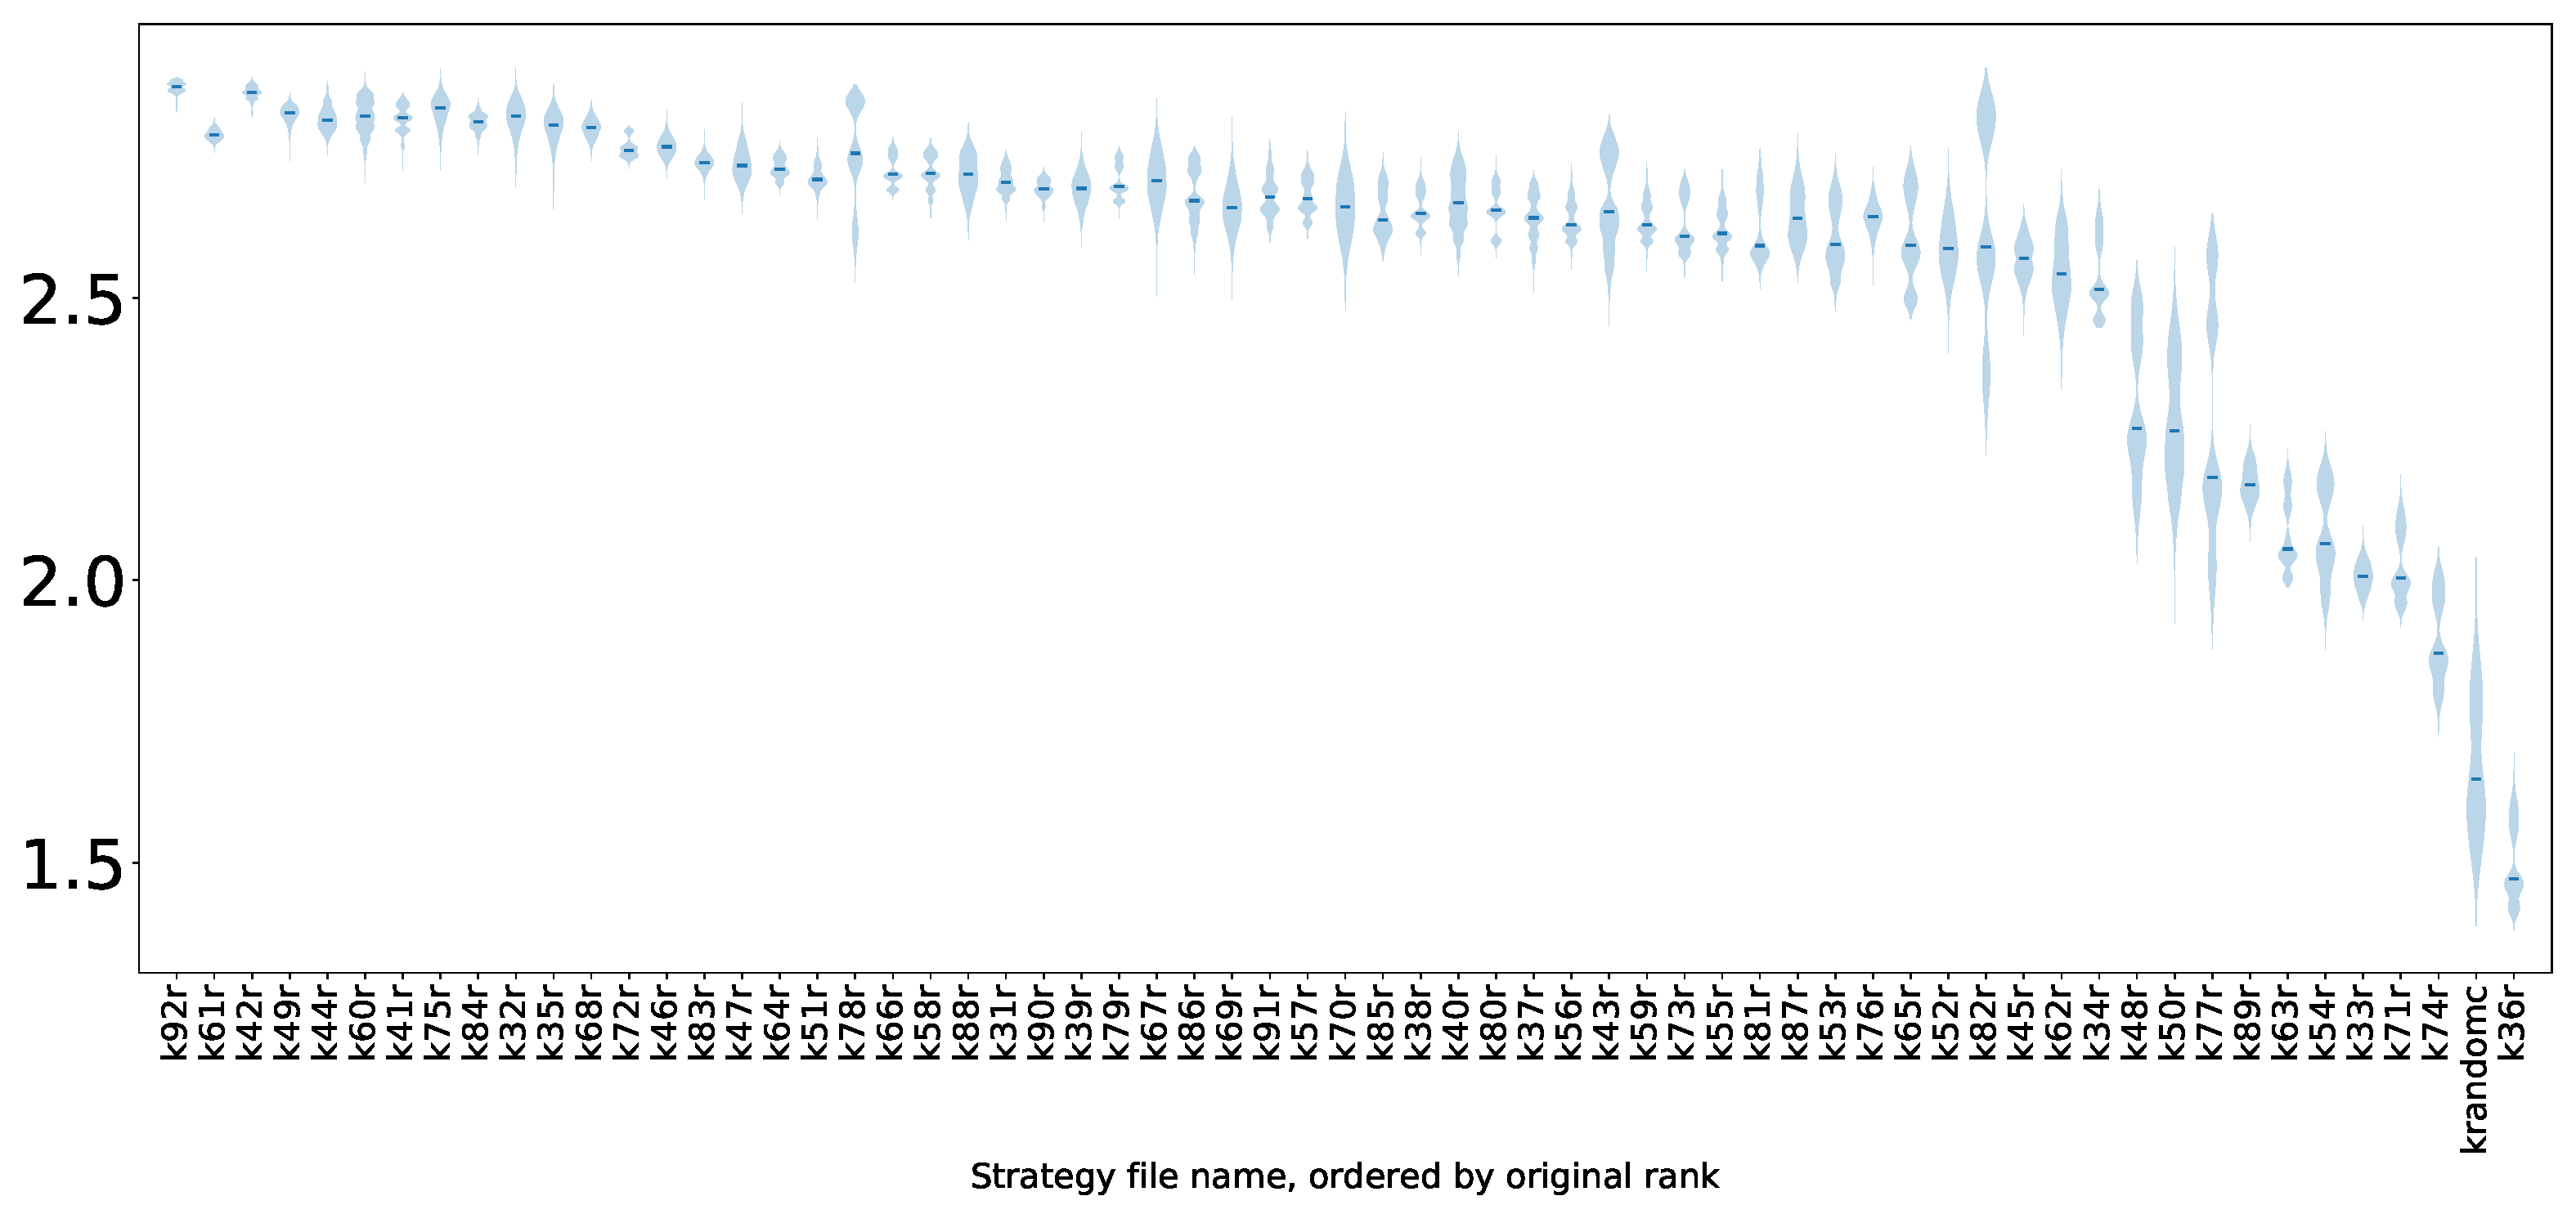
\includegraphics[width=.8\textwidth]{assets/original_scores_boxplots.pdf}
    \caption{The scores per turn of each strategy.}
    \label{fig:original_tournament_scores}
\end{figure}

Whilst the results mainly agree with the original reported results, some
strategies show distinct outliers:

\begin{itemize}
    \item k61r
    \item k90r
    \item k82r
\end{itemize}
% TODO Investigate

Note that there are various approaches to calculating the ranks/results,
Figure~\ref{fig:original_tournament_rankings} shows the rankings calculated in
various ways as well as the mean absolute error (MAE).

\begin{figure}[!hbtp]
    \centering
    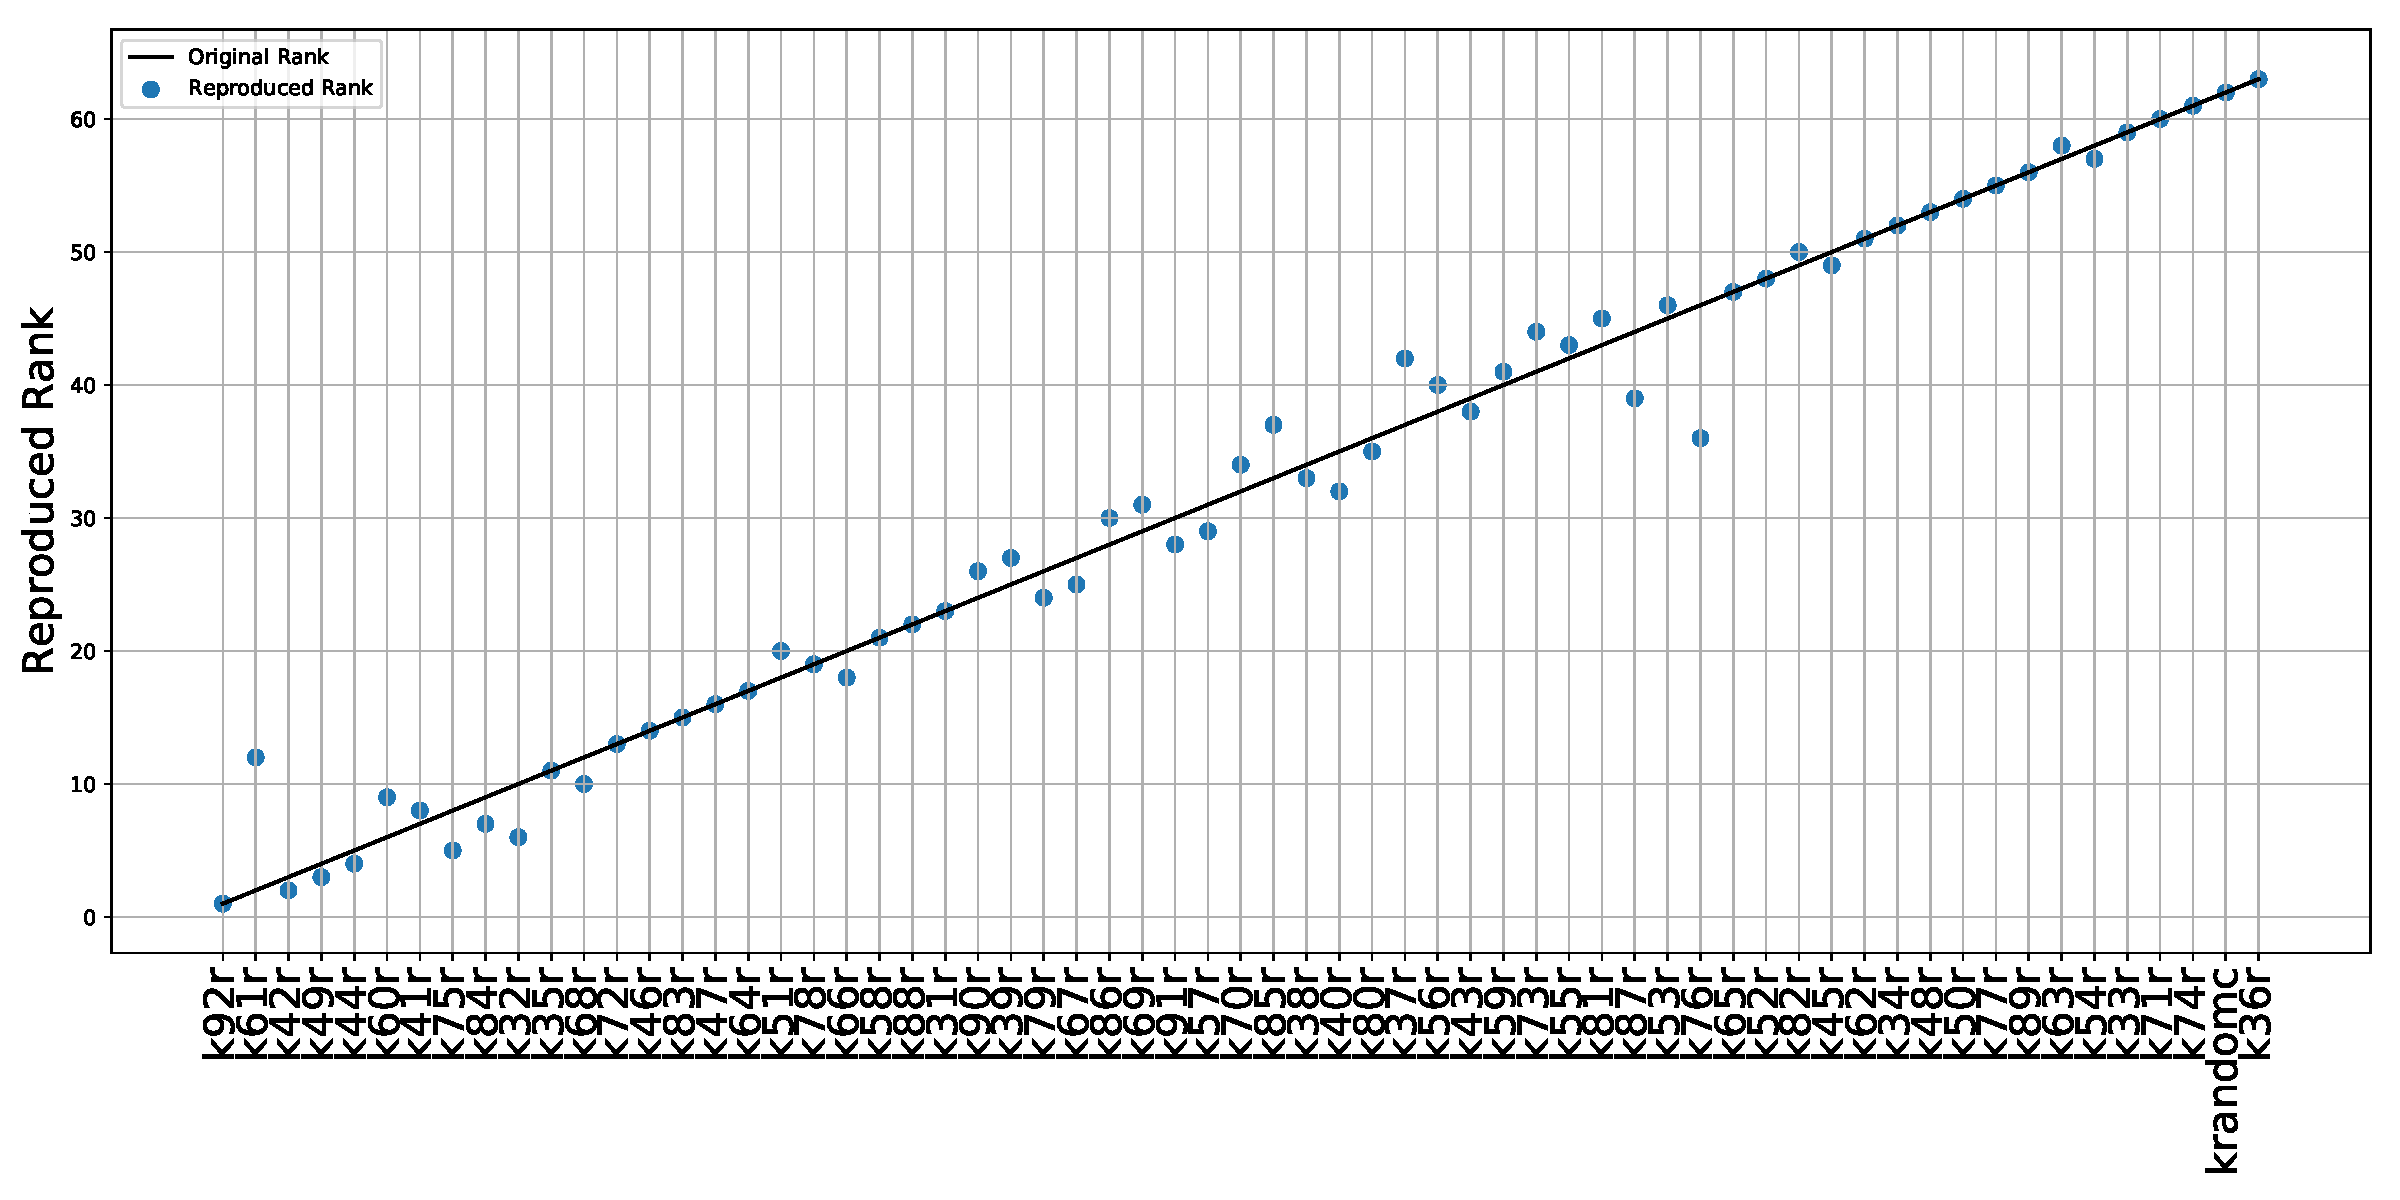
\includegraphics[width=.8\textwidth]{assets/original_tournament_rankings.pdf}
    \caption{The rankings of each strategy.}
    \label{fig:original_tournament_rankings}
\end{figure}

The top 15 strategies in the reproduced tournament are shown in
Table~\ref{tbl:original_tournament_rankings}.

\begin{table}[!hbtp]
        \centering
        \begin{tabular}{llrrr}
\toprule
{} &                                 Author &  Scores &  Rank &  Original Rank \\
\midrule
k92r &                        Anatol Rapoport &  2.8786 &     1 &              1 \\
k61r &                       Danny C Champion &  2.7189 &    17 &              2 \\
k42r &                          Otto Borufsen &  2.8342 &     2 &              3 \\
k49r &                               Rob Cave &  2.8259 &     4 &              4 \\
k44r &                          William Adams &  2.8262 &     3 &              5 \\
k60r &           Jim Graaskamp and Ken Katzen &  2.8103 &     9 &              6 \\
k41r &                            Herb Weiner &  2.8104 &     8 &              7 \\
k75r &                      Paul D Harrington &  2.8240 &     5 &              8 \\
k84r &  T Nicolaus Tideman and Paula Chieruzz &  2.8126 &     7 &              9 \\
k32r &                       Charles Kluepfel &  2.8164 &     6 &             10 \\
k35r &                        Abraham Getzler &  2.8018 &    11 &             11 \\
k68r &                       Fransois Leyvraz &  2.8088 &    10 &             12 \\
k72r &                      Edward C White Jr &  2.7766 &    12 &             13 \\
k46r &                     Graham J Eatherley &  2.7724 &    13 &             14 \\
k83r &                           Paul E Black &  2.7427 &    14 &             15 \\
\bottomrule
\end{tabular}

        \caption{Top 15 strategies in the reproduced tournament}
        \label{tbl:original_tournament_rankings}
\end{table}

In~\cite{Axelrod1980b}, a linear regression model is used to identify 5
strategies, the scores against which are good predictors of the overall
performance. The reported \(R^2\) value is \(0.979\) (indicating 97\% of
variance accounted for by the model). The coefficients of this model are shown
in Table~\ref{tbl:original_tournament_representative_model}.

\begin{table}[!hbtp]
        \centering
        \begin{tabular}{lr}
\toprule
Strategies & Coefficients \\
\midrule
k69r & 0.202000 \\
k91r & 0.198000 \\
k40r & 0.110000 \\
k76r & 0.072000 \\
k67r & 0.086000 \\
Intercept & 0.795000 \\
\bottomrule
\end{tabular}

        \caption{Linear model described in~\cite{Axelrod1980b} with
             \(R^2=\protect0.7508\)}
        \label{tbl:original_tournament_representative_model}
\end{table}

Given the discrepancy in results shown in
Figure~\ref{fig:original_tournament_rankings} and
Table~\ref{tbl:original_tournament_rankings} it is not surprising to see that
this model no longer performs as well with
\(R^2=0.7508\).

Fitting a new model to the same 5 strategies gives the coefficients shown in
Table~\ref{tbl:original_tournament_predictive_with_axelrod_5_model} with
\(R^2=0.9440\)

\begin{table}[!hbtp]
        \centering
        \begin{tabular}{lrll}
\toprule
Strategies & Coefficients & $p$-value & $F$-value \\
\midrule
k69r & 0.098640 & 0.000000 & 43.976036 \\
k91r & 0.207380 & 0.000000 & 56.667196 \\
k40r & 0.206440 & 0.000000 & 78.191831 \\
k76r & 0.059930 & 0.025992 & 5.207451 \\
k67r & 0.123740 & 0.000002 & 27.893148 \\
Intercept & 0.768410 & NA & NA \\
\bottomrule
\end{tabular}

        \caption{Linear model fitted to the same 5 strategies described
                 in~\cite{Axelrod1980b} with
             \(R^2=\protect0.9440\)}
        \label{tbl:original_tournament_predictive_with_axelrod_5_model}
\end{table}

Using recursive feature elimination
% TODO Include a text book reference
It is possible to select the features (strategies) that give the best prediction
for a given number of features. The \(R^2\) versus the number of features is
shown in
Figure~\ref{fig:original_tournament_r_squared_versus_number_of_features}.

\begin{figure}[!hbtp]
    \centering
    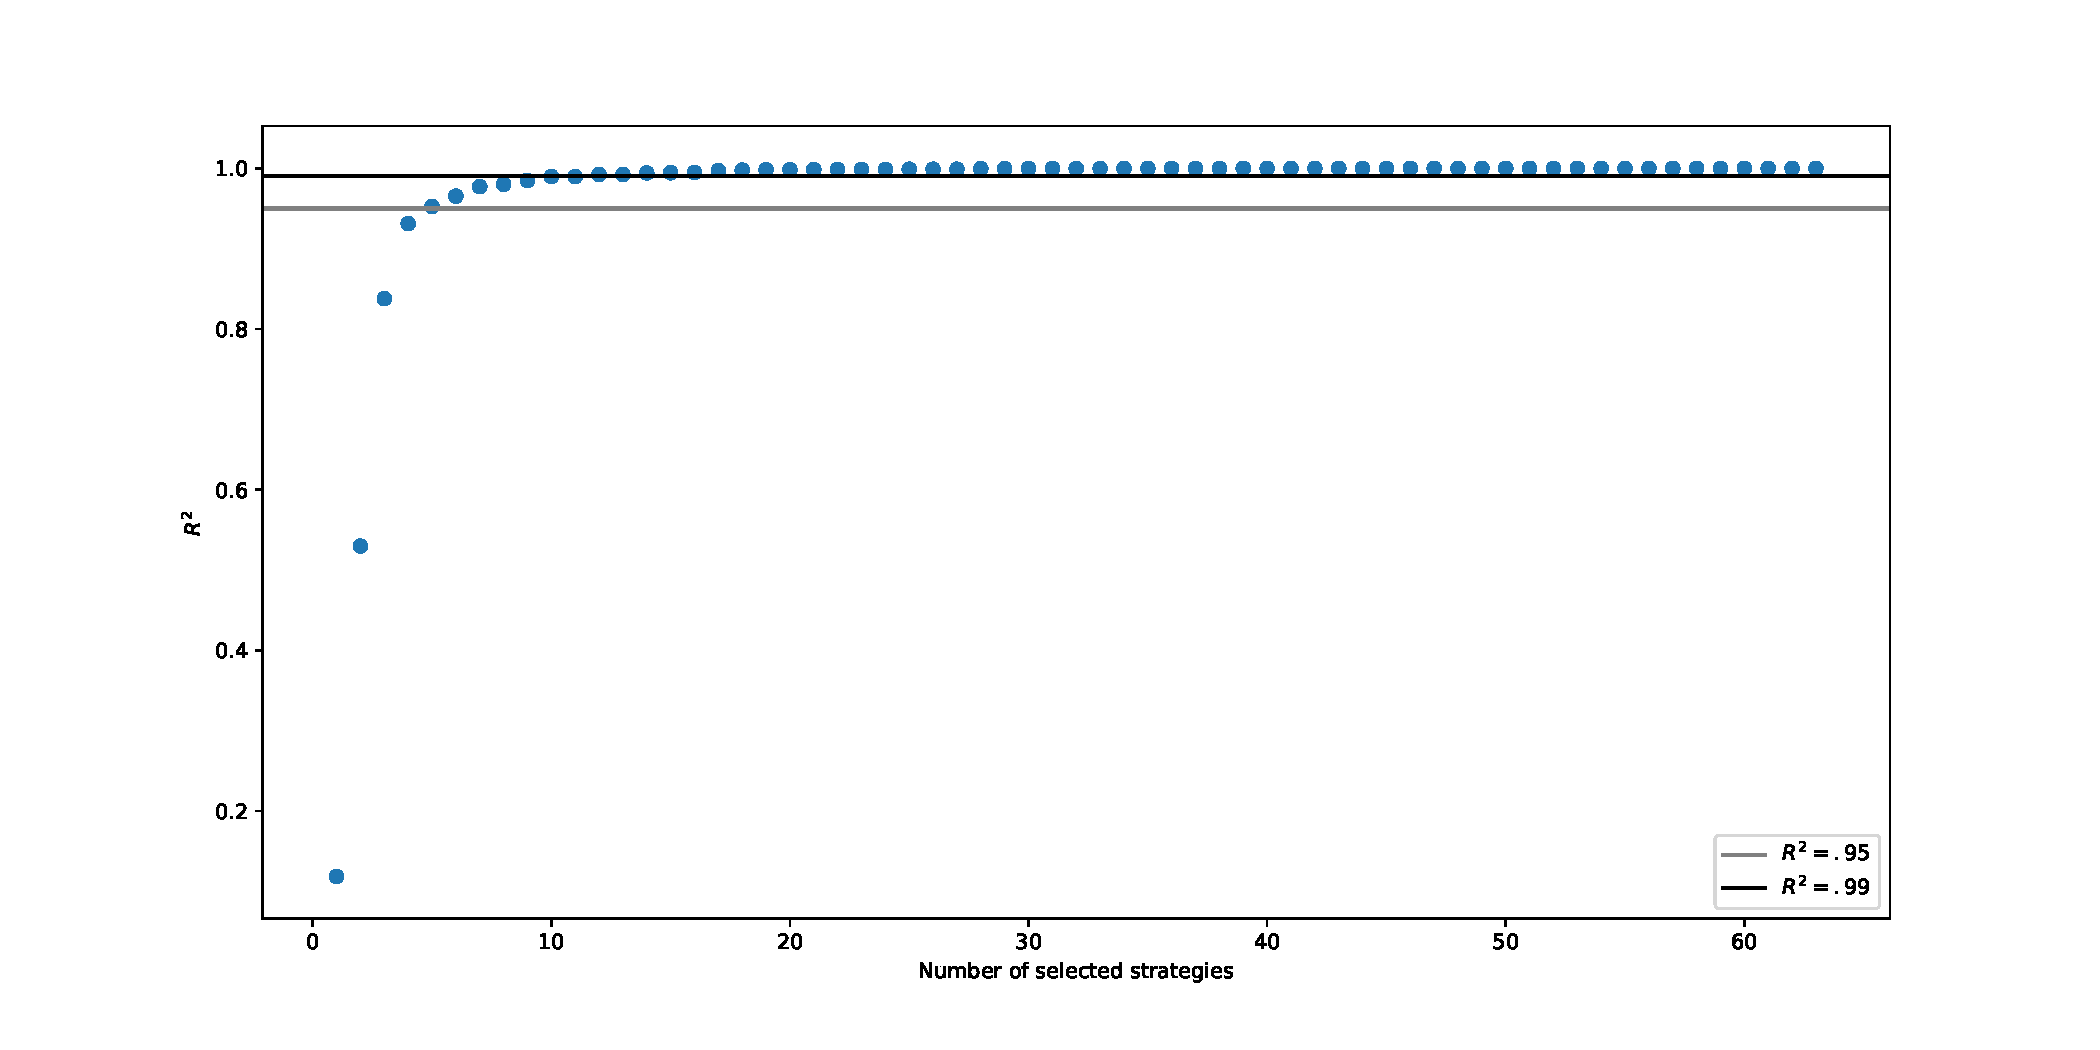
\includegraphics[width=.8\textwidth]{assets/original_tournament_r_squared_versus_number_of_features.pdf}
    \caption{\(R^2\) for models obtained using recursive feature elimination.}
    \label{fig:original_tournament_r_squared_versus_number_of_features}
\end{figure}


Tables~\ref{tbl:original_tournament_predictive_5_model}
and~\ref{tbl:original_tournament_predictive_12_model} show the coefficients for
linear models fitted to 5 and 12 strategies with
\(R^2=0.9440\) and
\(R^2=0.9930\)
respectively (12 strategies is the smallest number of strategies for which
\(R^2>95\).


\begin{table}[!hbtp]
        \centering
        \begin{tabular}{lrll}
\toprule
Strategies &  Coefficients &    $p$-value & $F$-value \\
\midrule
      k55r &         0.191 &  5.20963e-08 &   38.5403 \\
      k73r &         0.165 &  2.42582e-11 &   66.4276 \\
      k82r &         0.134 &  1.80697e-06 &   27.8953 \\
      k84r &         0.092 &  6.31455e-18 &   147.489 \\
      k92r &         0.188 &  2.68503e-13 &    86.435 \\
 Intercept &         0.520 &           NA &        NA \\
\bottomrule
\end{tabular}

        \caption{Linear model best fitted to 5 strategies in the reproduced tournament
                 with
             \(R^2=\protect0.9440\)}
        \label{tbl:original_tournament_predictive_5_model}
\end{table}

\begin{table}[!hbtp]
        \centering
        \begin{tabular}{lrll}
\toprule
Strategies &  Coefficients &    $p$-value & $F$-value \\
\midrule
      k31r &         0.166 &  5.15065e-05 &   18.9782 \\
      k34r &         0.081 &  1.39931e-08 &   42.8242 \\
      k51r &         0.230 &   0.00357868 &    9.1841 \\
      k52r &         0.116 &     0.572461 &   0.32205 \\
      k56r &        -1.695 &   1.2278e-09 &   51.2719 \\
      k59r &         1.729 &   1.2399e-09 &   51.2364 \\
      k64r &        -0.150 &  2.41824e-14 &   98.4147 \\
      k79r &         0.121 &  2.36814e-14 &   98.5231 \\
      k82r &         0.120 &  1.08815e-06 &   29.3393 \\
      k84r &         0.220 &  9.37609e-18 &   144.822 \\
      k88r &         0.112 &   1.8614e-15 &   112.266 \\
      k91r &         0.066 &  2.50396e-10 &   57.1748 \\
 Intercept &        -0.485 &           NA &        NA \\
\bottomrule
\end{tabular}

        \caption{Linear model best fitted to 12 strategies in the reproduced tournament
                 with
             \(R^2=\protect0.9930\)}
        \label{tbl:original_tournament_predictive_12_model}
\end{table}

The predictions of these models are shown in
Figure~\ref{fig:original_tournament_predictive_score_models}.

\begin{figure}[!hbtp]
    \centering
    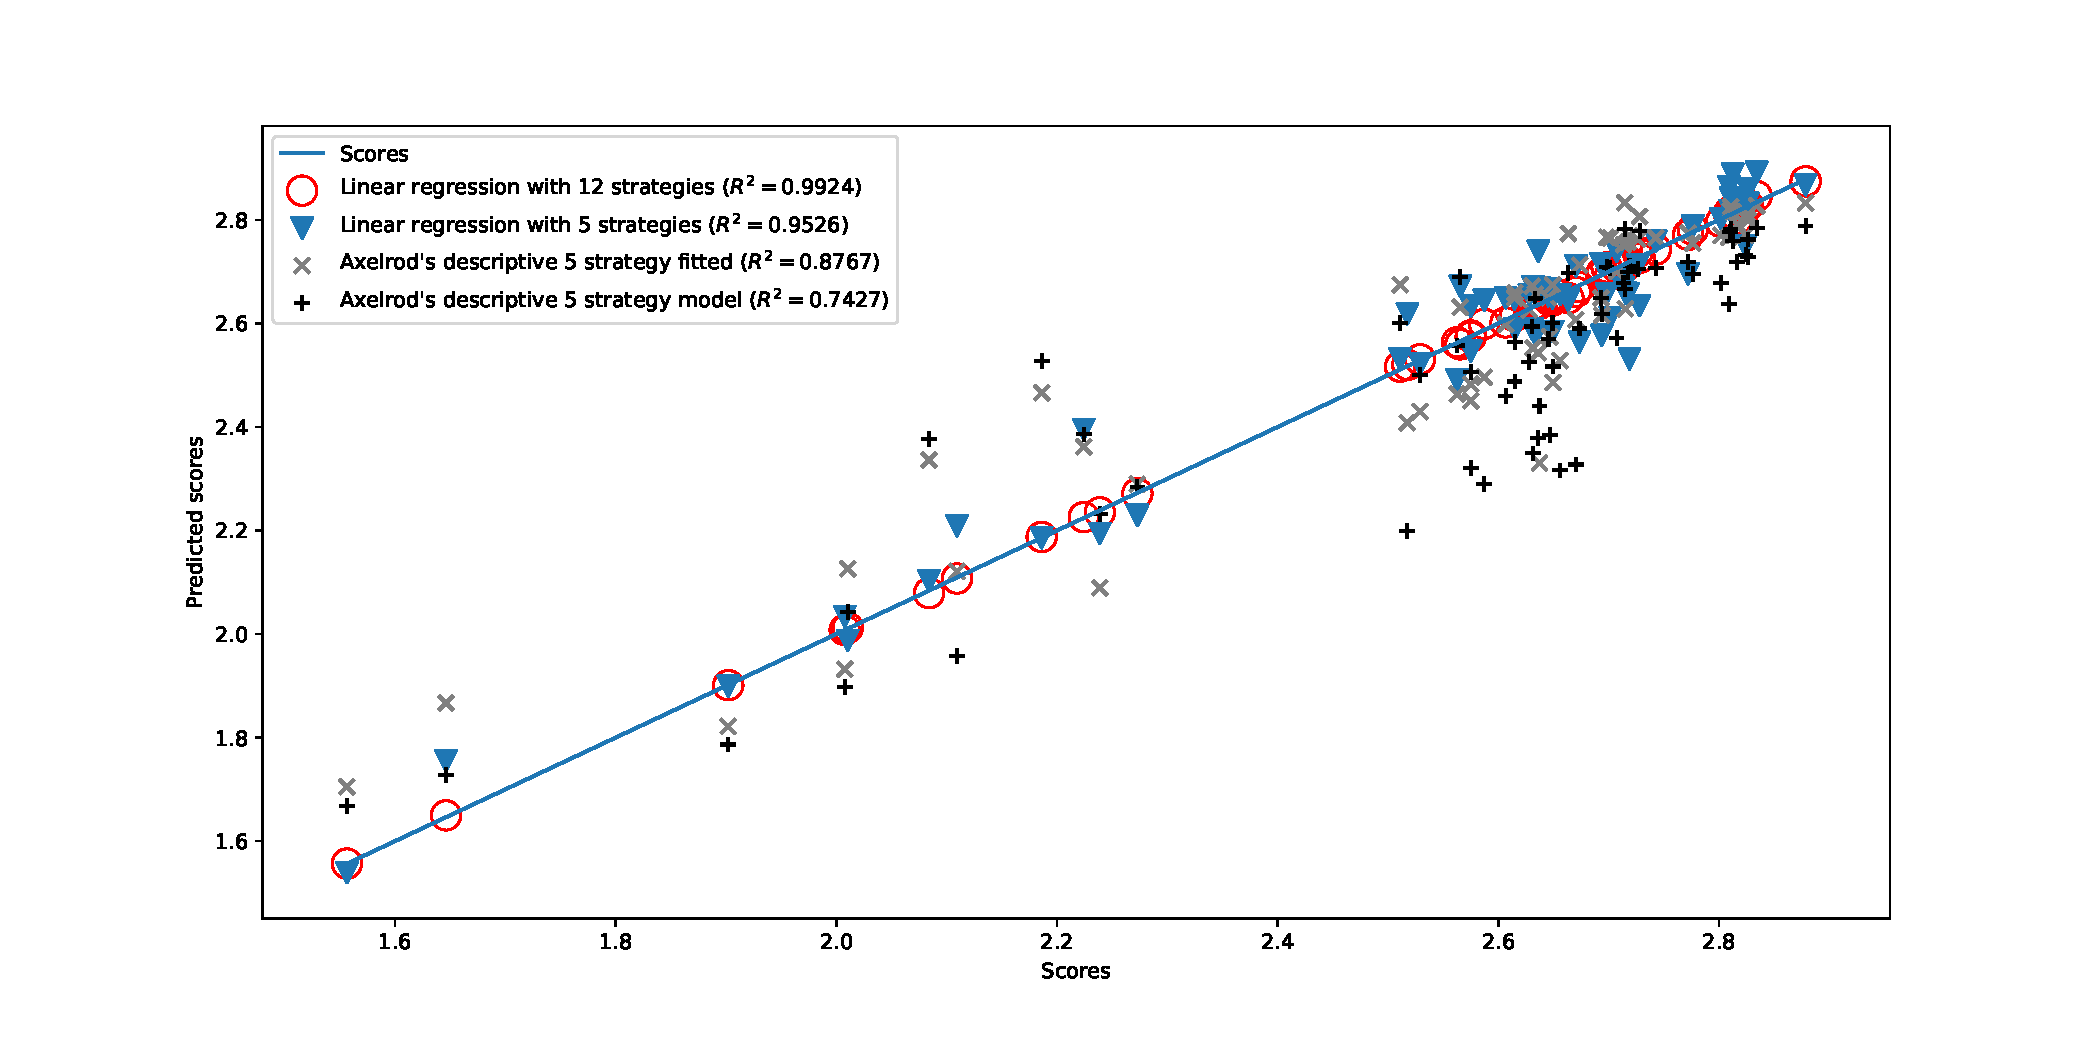
\includegraphics[width=.8\textwidth]{assets/original_tournament_predictive_score_models.pdf}
    \caption{Predicting the performance of strategies using the 4 models
             discussed}
    \label{fig:original_tournament_predictive_score_models}
\end{figure}

It is clear that the effectiveness of the predictive models with 5 strategies is
low for the cluster of highly performing strategies (with a score great than
2.5). To be able to obtain a good model even for high performing strategies 12
seem to provide a good predictive model.

The overall cooperation rate of the tournament
is 0.750.
Figure~\ref{fig:original_tournament_cooperation_rate_versus_rank} shows the
cooperation rate versus the rank of the strategy.

\begin{figure}[!hbtp]
    \centering
    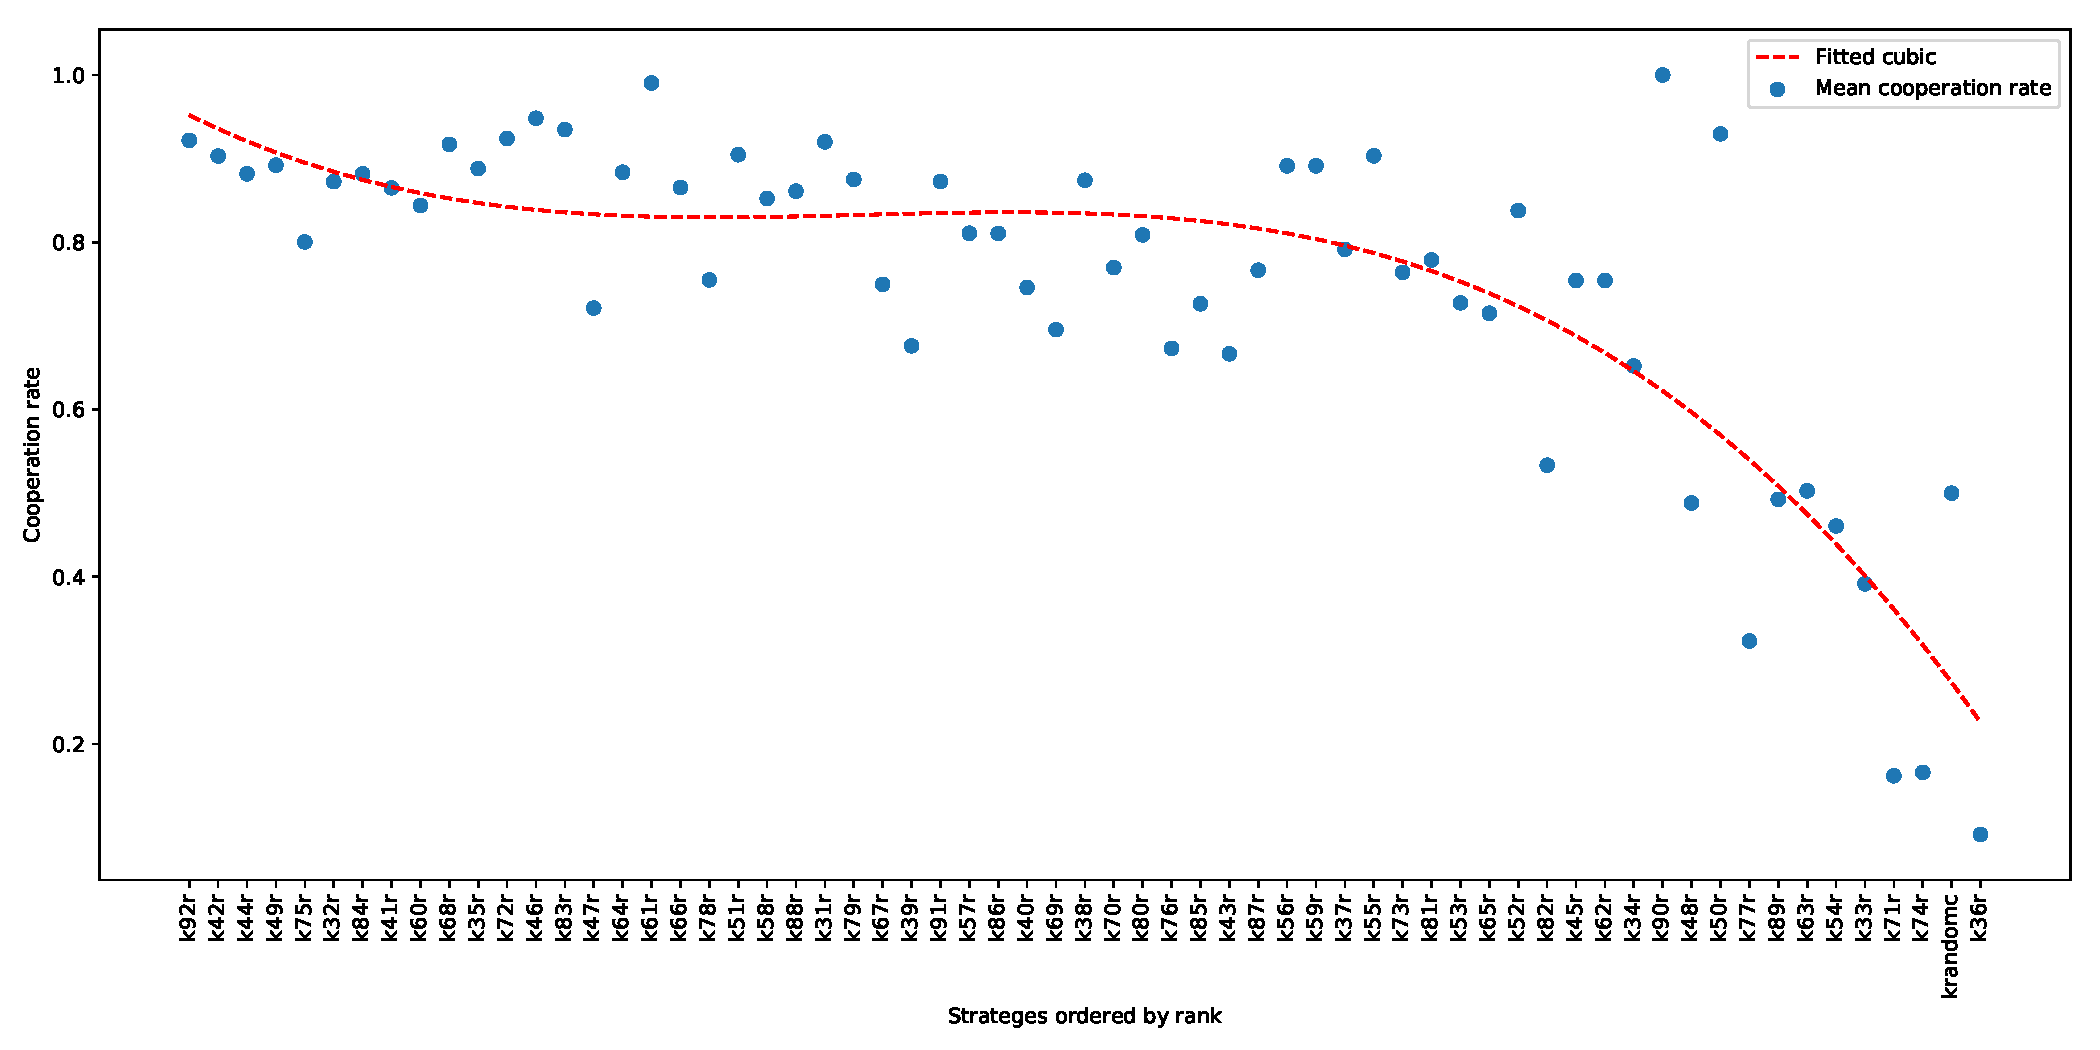
\includegraphics[width=.8\textwidth]{assets/original_tournament_cooperation_rate_versus_rank.pdf}
    \caption{Cooperation rate versus rank}
    \label{fig:original_tournament_cooperation_rate_versus_rank}
\end{figure}



\begin{figure}[!hbtp]
    \centering
    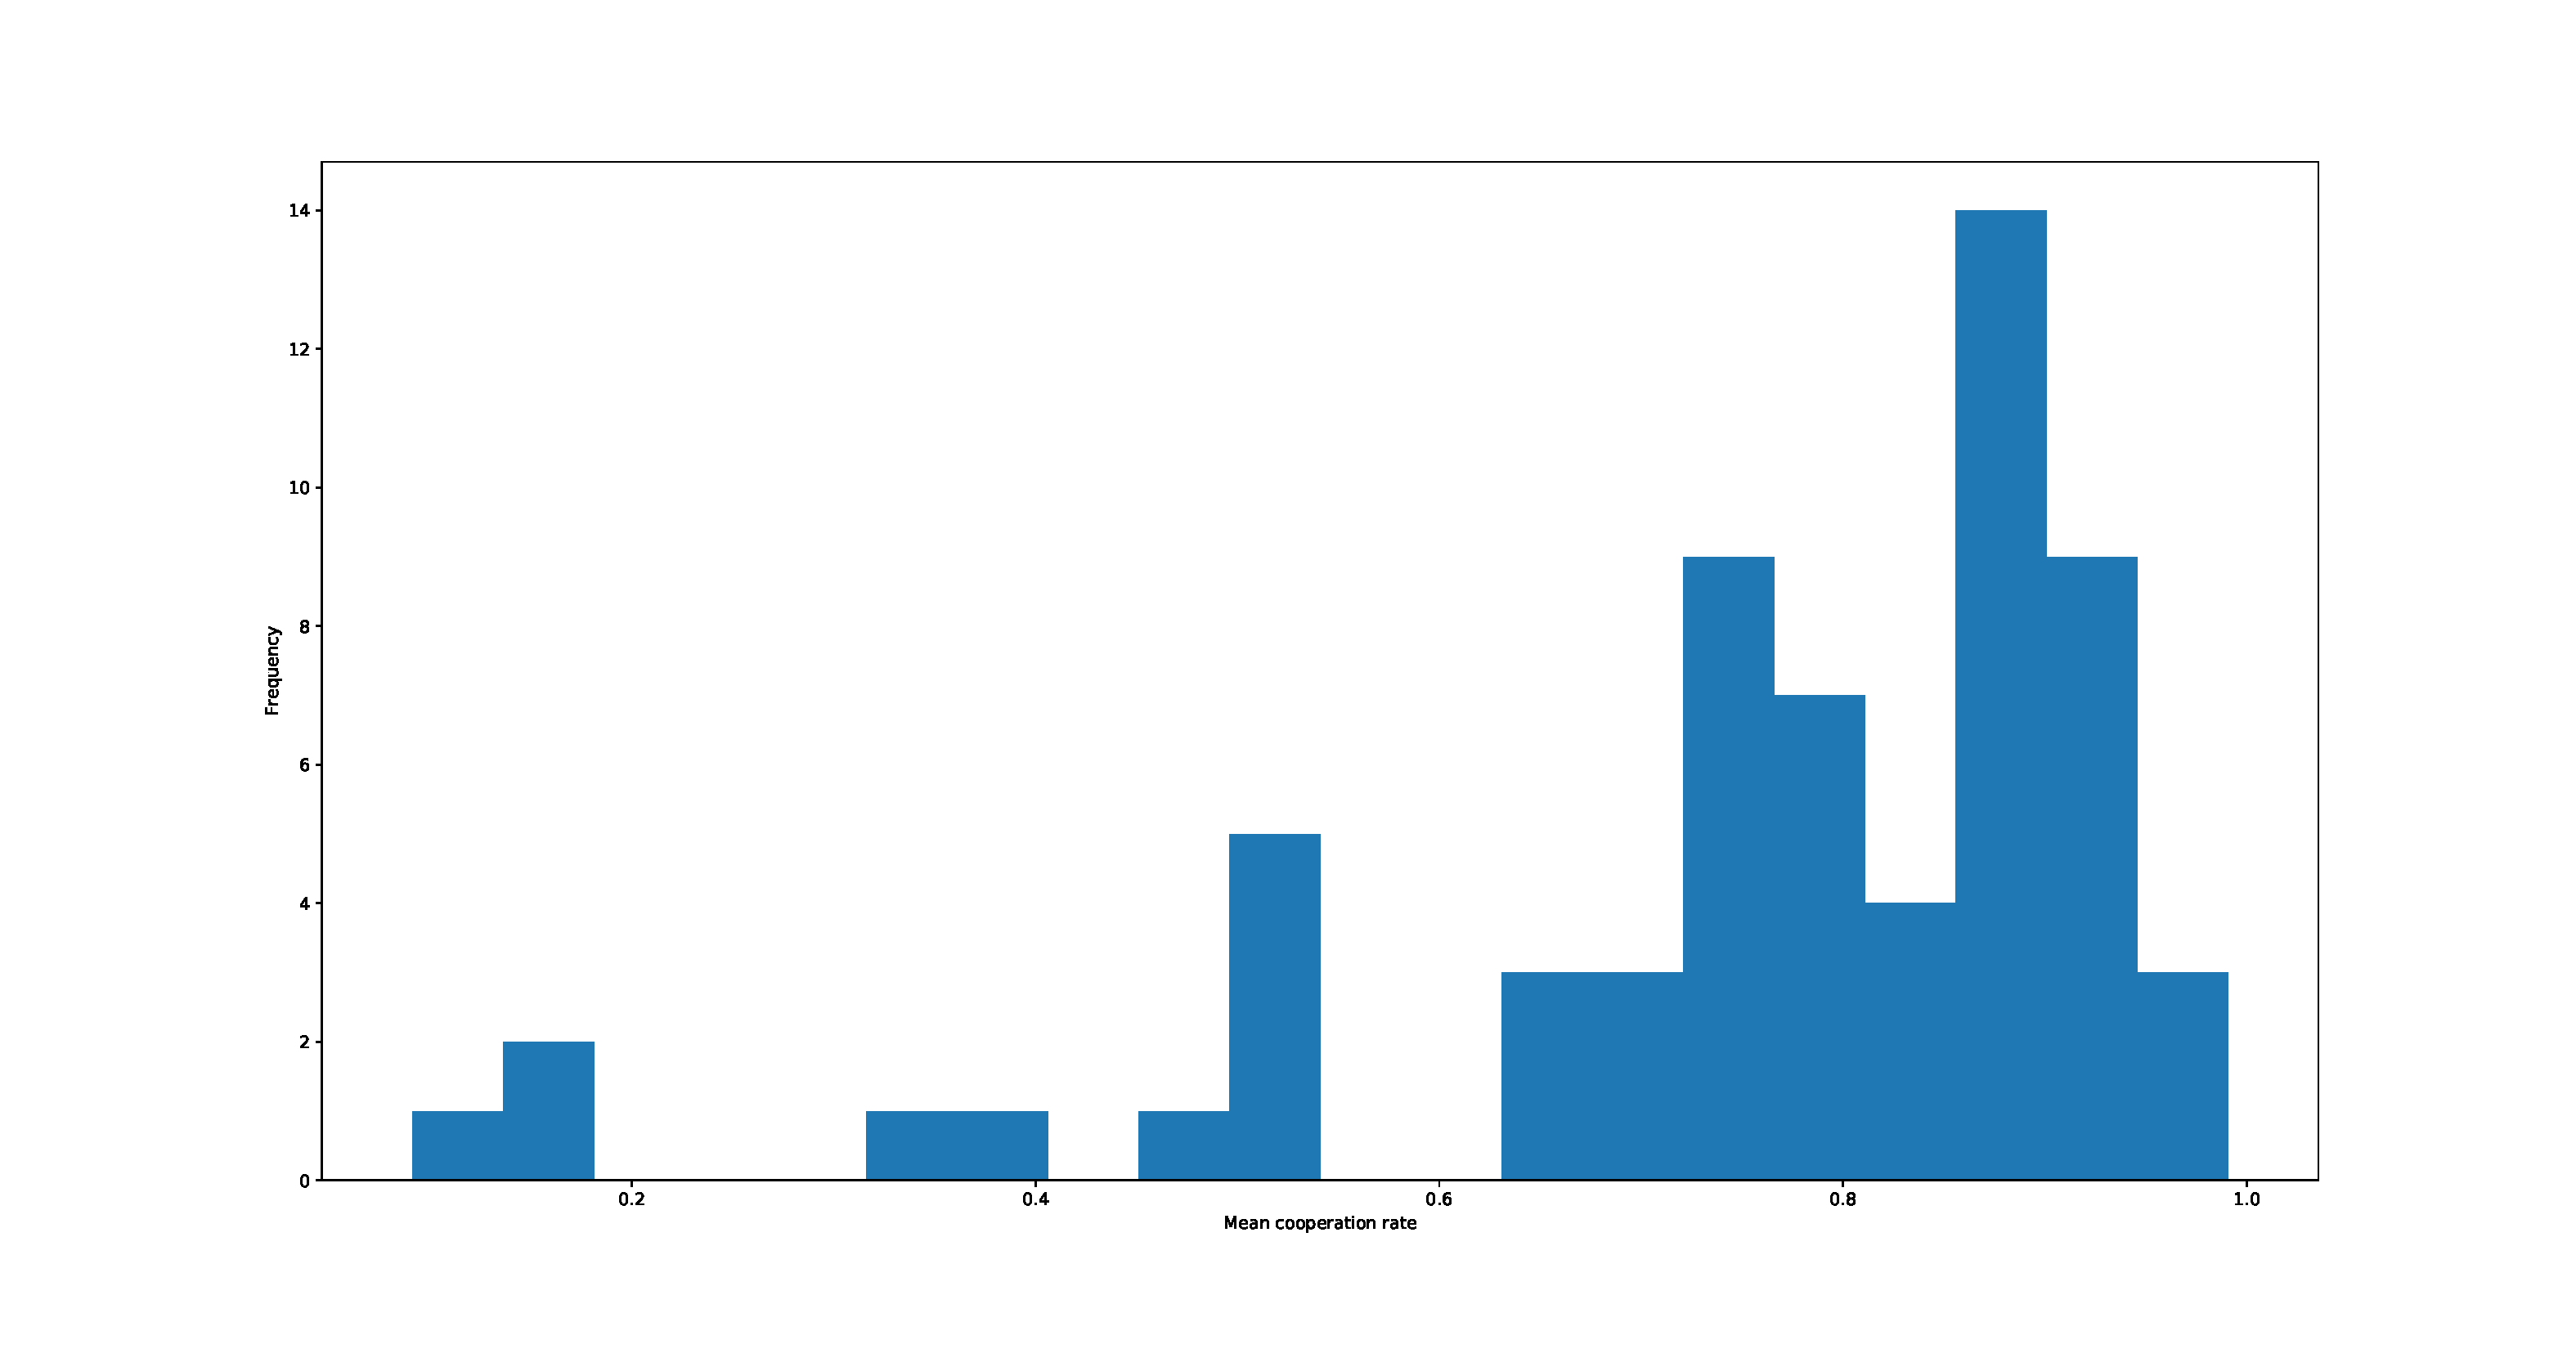
\includegraphics[width=.8\textwidth]{assets/original_tournament_cooperation_rates.pdf}
    \caption{Distribution of cooperation rates}
    \label{fig:original_tournament_cooperation_rates}
\end{figure}

Figure~\ref{fig:original_tournament_pairwise_cooperation_rates} shows the pair wise
cooperation rates. There is one strategy `k42r' that defects against itself but
cooperates against most other strategies. Also, it is clear that the low
performing strategies are defecting against each other.

\begin{figure}[!hbtp]
    \centering
    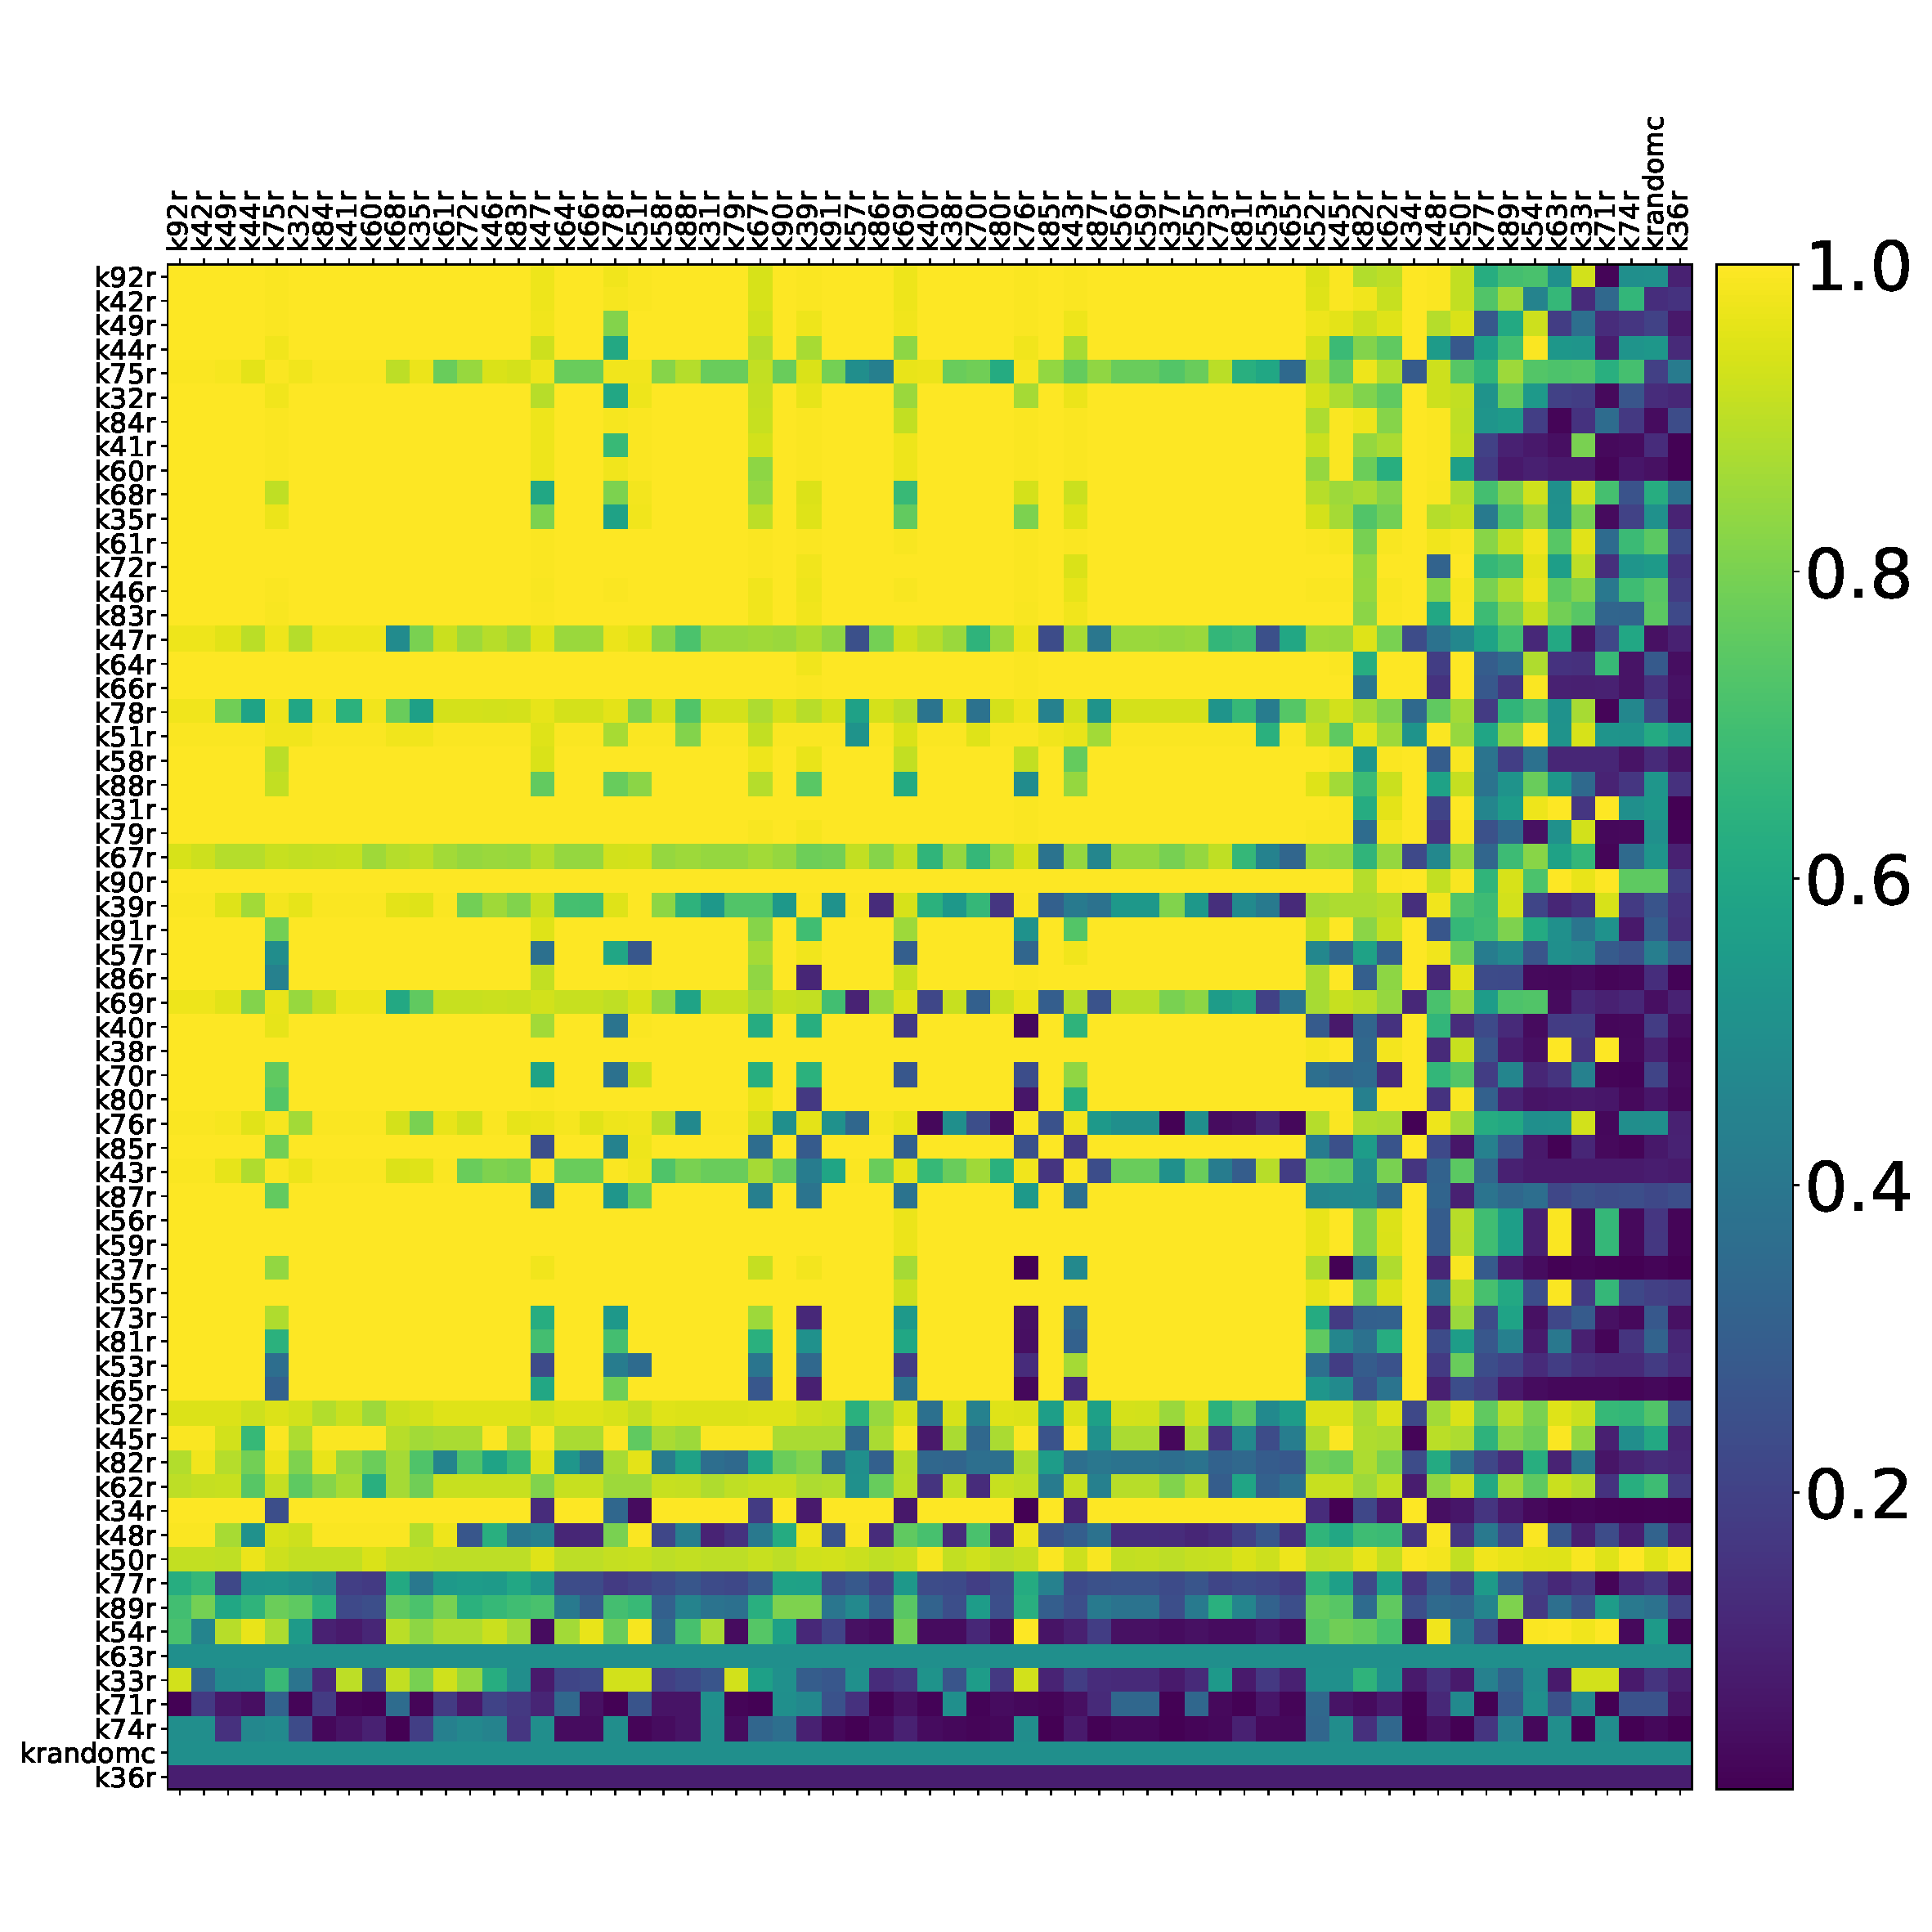
\includegraphics[width=.8\textwidth]{assets/original_tournament_pairwise_cooperation_rates.pdf}
    \caption{Cooperation rates between each pair of players (ordered by rank)}
    \label{fig:original_tournament_pairwise_cooperation_rates}
\end{figure}


\section{Revisiting the tournament}\label{sec:revisiting}

\subsection{Running with an extra invitation}\label{sec:extra_strategy}

\subsubsection{Known strategies}

The tournament is run with every strategy of the Axelrod library.
% TODO Cite properly
% TODO Point at appendix
Every tournament (corresponding to each strategy) was run
for 4000repetitions.
Table~\ref{tbl:original_tournament_with_extra_strategy_summary} shows the top
ranking strategies.

\begin{table}[!hbtp]
        \footnotesize
        \centering
        \begin{tabular}{lrrl}
\toprule
 & Mean Score & Rank & Winner \\
Name &  &  &  \\
\midrule
Adaptive Tit For Tat: 0.5 & 2.876 & 2 & k92r \\
GTFT: 0.33 & 2.846 & 3 & k92r \\
Omega TFT: 3, 8 & 2.859 & 3 & k92r \\
Firm But Fair & 2.861 & 3 & k92r \\
ZD-GTFT-2: 0.25, 0.5 & 2.868 & 3 & k92r \\
Resurrection & 2.867 & 3 & k92r \\
Meta Majority: 213 players & 2.860 & 3 & k92r \\
Meta Majority Finite Memory: 79 players & 2.856 & 3 & k92r \\
Meta Majority Long Memory: 134 players & 2.856 & 3 & k92r \\
Soft Joss: 0.9 & 2.871 & 3 & k92r \\
Forgiving Tit For Tat & 2.854 & 3 & k92r \\
Original Gradual & 2.857 & 3 & k92r \\
Meta Majority Memory One: 36 players & 2.838 & 4 & k92r \\
PSO Gambler 2\_2\_2 Noise 05 & 2.840 & 4 & k92r \\
Gradual & 2.831 & 7 & k92r \\
First by Stein and Rapoport: 0.05: (D, D) & 2.827 & 8 & k92r \\
Spiteful Tit For Tat & 2.826 & 8 & k92r \\
GrudgerAlternator & 2.825 & 8 & k92r \\
EugineNier: (D,) & 2.815 & 10 & k92r \\
First by Shubik & 2.791 & 13 & k92r \\
\bottomrule
\end{tabular}

        \caption{Performance of extra strategy in Axelrod's original tournament}
        \label{tbl:original_tournament_with_extra_strategy_summary}
\end{table}

Figure~\ref{fig:original_tournament_with_extra_strategy_ranks_vs_library_ranks}
shows the rank of the extra strategy against it's rank in the library
tournament.

\begin{figure}[!hbtp]
    \centering
    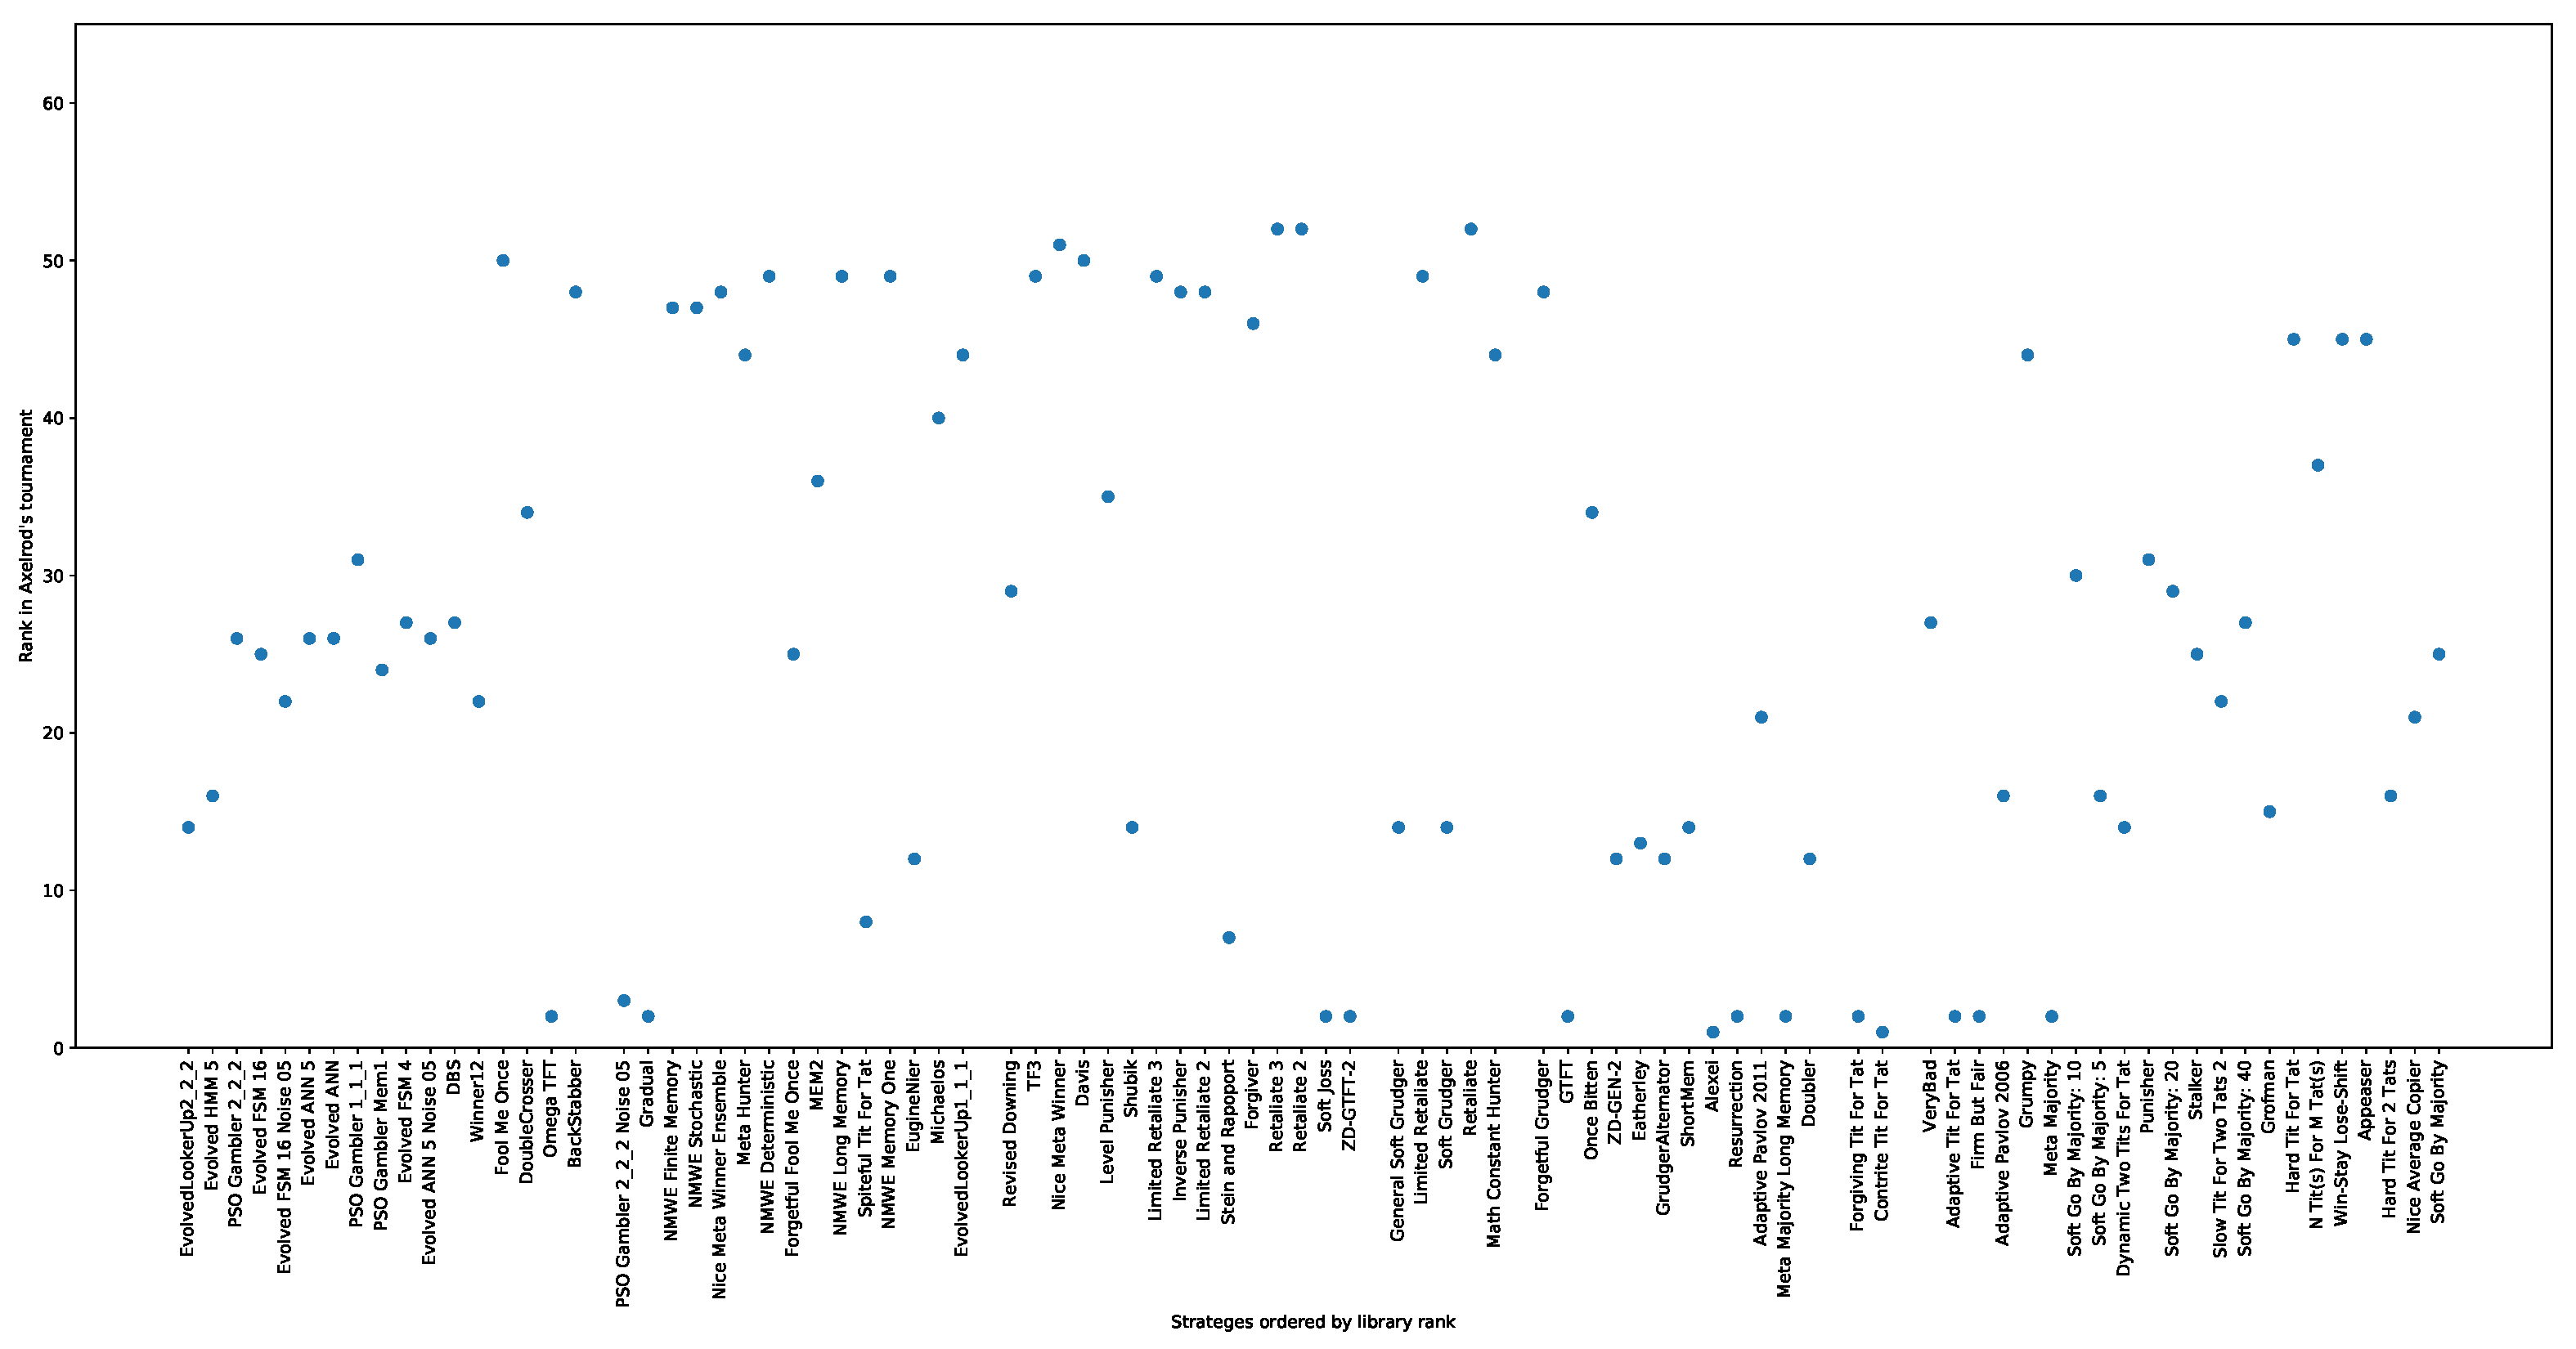
\includegraphics[width=.8\textwidth]{assets/original_tournament_with_extra_strategy_ranks_vs_library_ranks.pdf}
    \caption{Ranks of extra strategy}
    \label{fig:original_tournament_with_extra_strategy_ranks_vs_library_ranks}
\end{figure}

\subsubsection{Trained strategies}

Using the various strategy sets and weights from the previous regression
analysis
% TODO Improve how this points and refers to training
it is possible to train strategies to compete in the tournament.
% TODO Add details about training (software + algorithm): also include a diagram
% about process
Figure~\ref{fig:training_data_max_score} show the mean utility of the strategies
trained for this work. The strategies trained are 10 state Finite State
machines.
% TODO Include references.
% TODO Draw final fsm ones.

\begin{figure}[!hbtp]
    \centering
    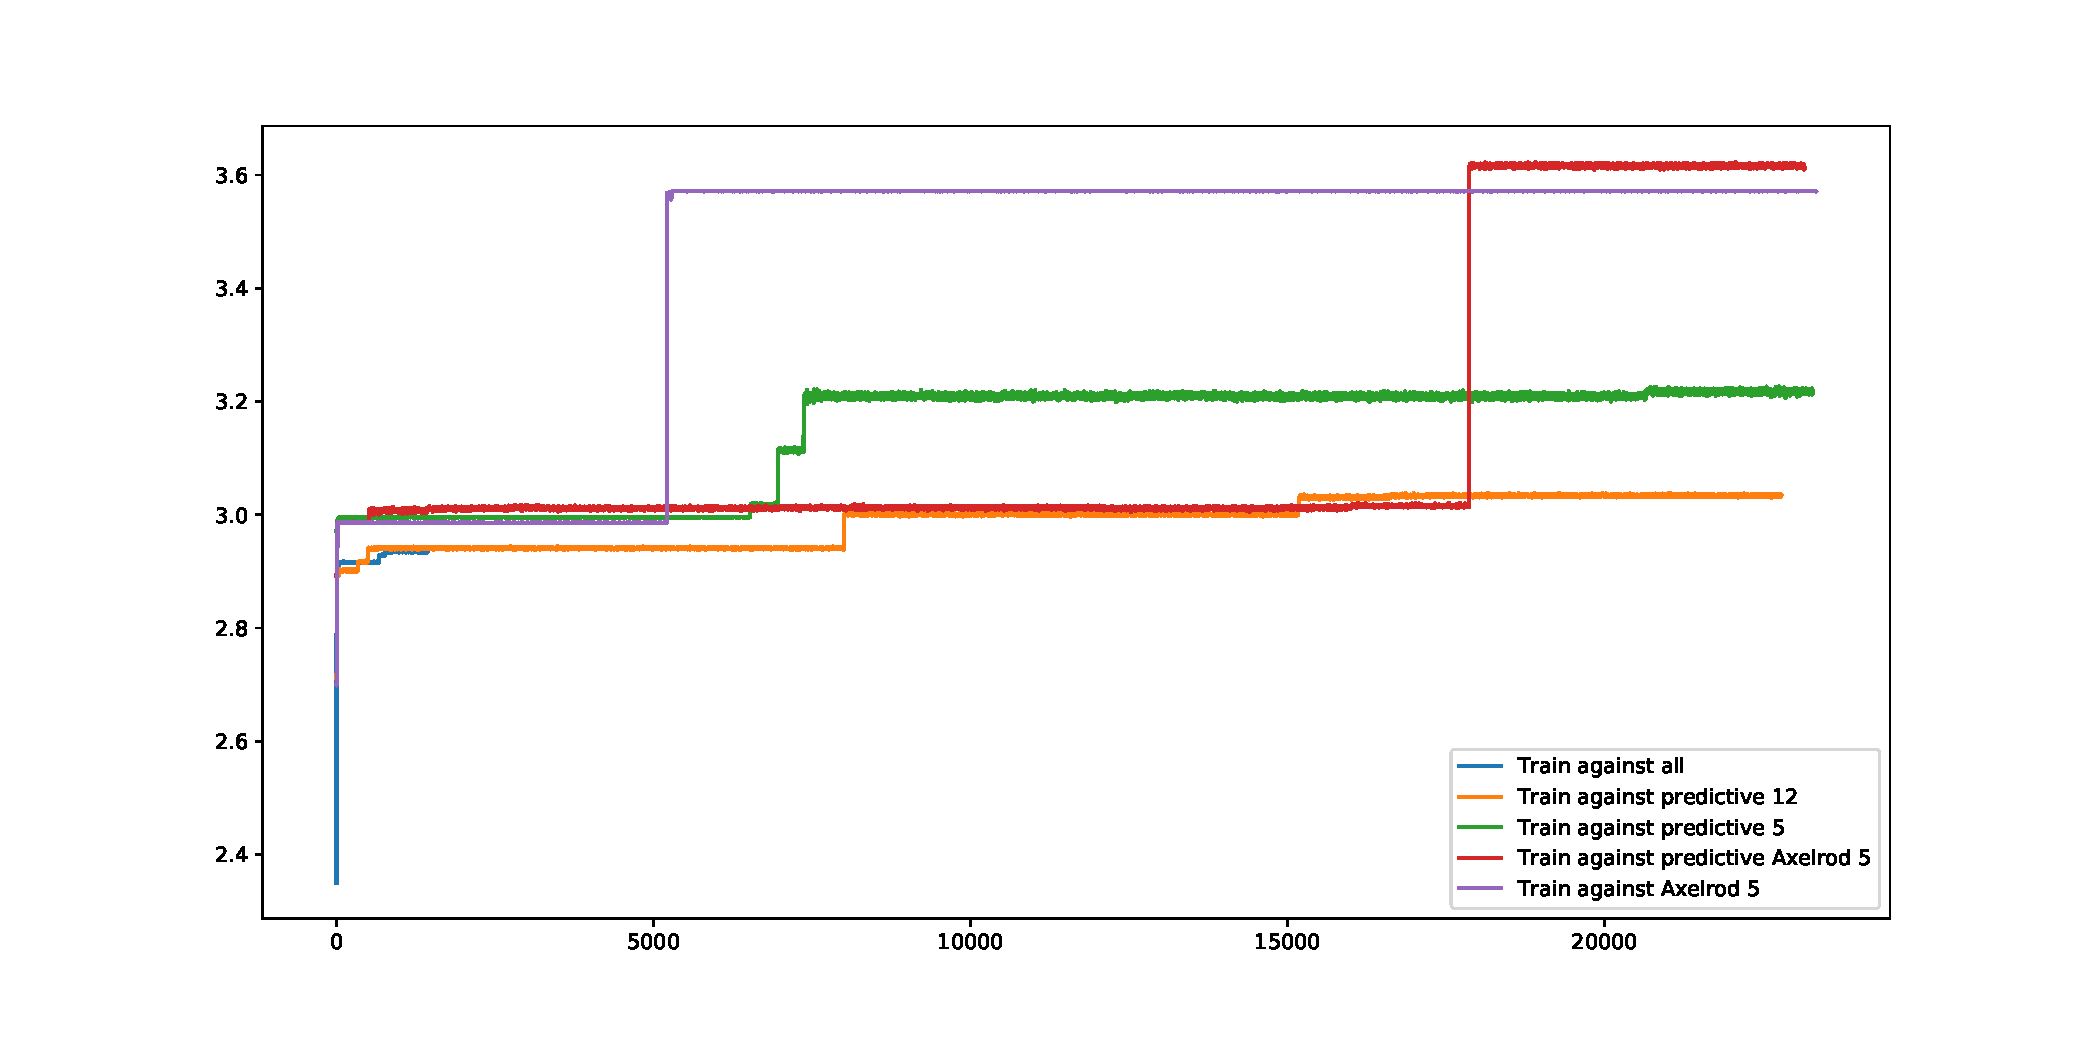
\includegraphics[width=.8\textwidth]{assets/training_data_max_score.pdf}
    \caption{The maximum score per generation over the training periods}
    \label{fig:training_data_max_score}
\end{figure}

The relative score is not necessarily interpretable (the weights of the
particular regression model skew this).
% TODO Add more details

% TODO Show results of trained strategies in tournaments.

\subsection{Further tournaments}

% TODO As a brief conclusion show results for these two larger tournaments.

\subsubsection{Running with extortion}\label{sec:run_with_stewart_plotkin}

Since the work of~\cite{Press2012} a lot of interest has been shown to Zero
Determinant strategies. In~\cite{Stewart2012} a small tournament is presented
pitting these against each other. Table~\ref{tbl:sp_tournament_rankings}
shows the rankings of the top 15 strategies when including all the Zero
Determinant strategies from~\cite{Stewart2012} over
25000repetitions.

\begin{table}[!hbtp]
        \centering
        \begin{tabular}{llrrrl}
\toprule
{} &                        Original Author &  Scores &  Rank &  Original Rank & Reproduced Rank \\
\midrule
ZD-GTFT-2 &                                     NA &  2.8366 &     1 &             NA &              NA \\
GTFT      &                                     NA &  2.8214 &     2 &             NA &              NA \\
k92r      &                        Anatol Rapoport &  2.8146 &     3 &              1 &               1 \\
k42r      &                          Otto Borufsen &  2.8046 &     4 &              3 &               2 \\
k75r      &                      Paul D Harrington &  2.7935 &     5 &              8 &               5 \\
k49r      &                               Rob Cave &  2.7894 &     6 &              4 &               4 \\
k44r      &                          William Adams &  2.7840 &     7 &              5 &               3 \\
k68r      &                       Fransois Leyvraz &  2.7717 &     8 &             12 &              10 \\
k41r      &                            Herb Weiner &  2.7648 &     9 &              7 &               8 \\
k32r      &                       Charles Kluepfel &  2.7617 &    10 &             10 &               6 \\
k46r      &                     Graham J Eatherley &  2.7614 &    11 &             14 &              13 \\
k72r      &                      Edward C White Jr &  2.7589 &    12 &             13 &              12 \\
k35r      &                        Abraham Getzler &  2.7506 &    13 &             11 &              11 \\
k84r      &  T Nicolaus Tideman and Paula Chieruzz &  2.7492 &    14 &              9 &               7 \\
k60r      &           Jim Graaskamp and Ken Katzen &  2.7382 &    15 &              6 &               9 \\
\bottomrule
\end{tabular}

        \caption{Top 15 strategies in the tournament composed of the original
                 strategies and the Zero Determinant strategies
                 from~\cite{Stewart2012}}
        \label{tbl:sp_tournament_rankings}
\end{table}

The overall cooperation rate of this tournament is
0.732and the various
cooperation rates are shown in
Figure~\ref{fig:sp_tournament_cooperation_rate_versus_rank} shows the
cooperation rates of each strategy (ordered by rank).

\begin{figure}[!hbtp]
    \centering
    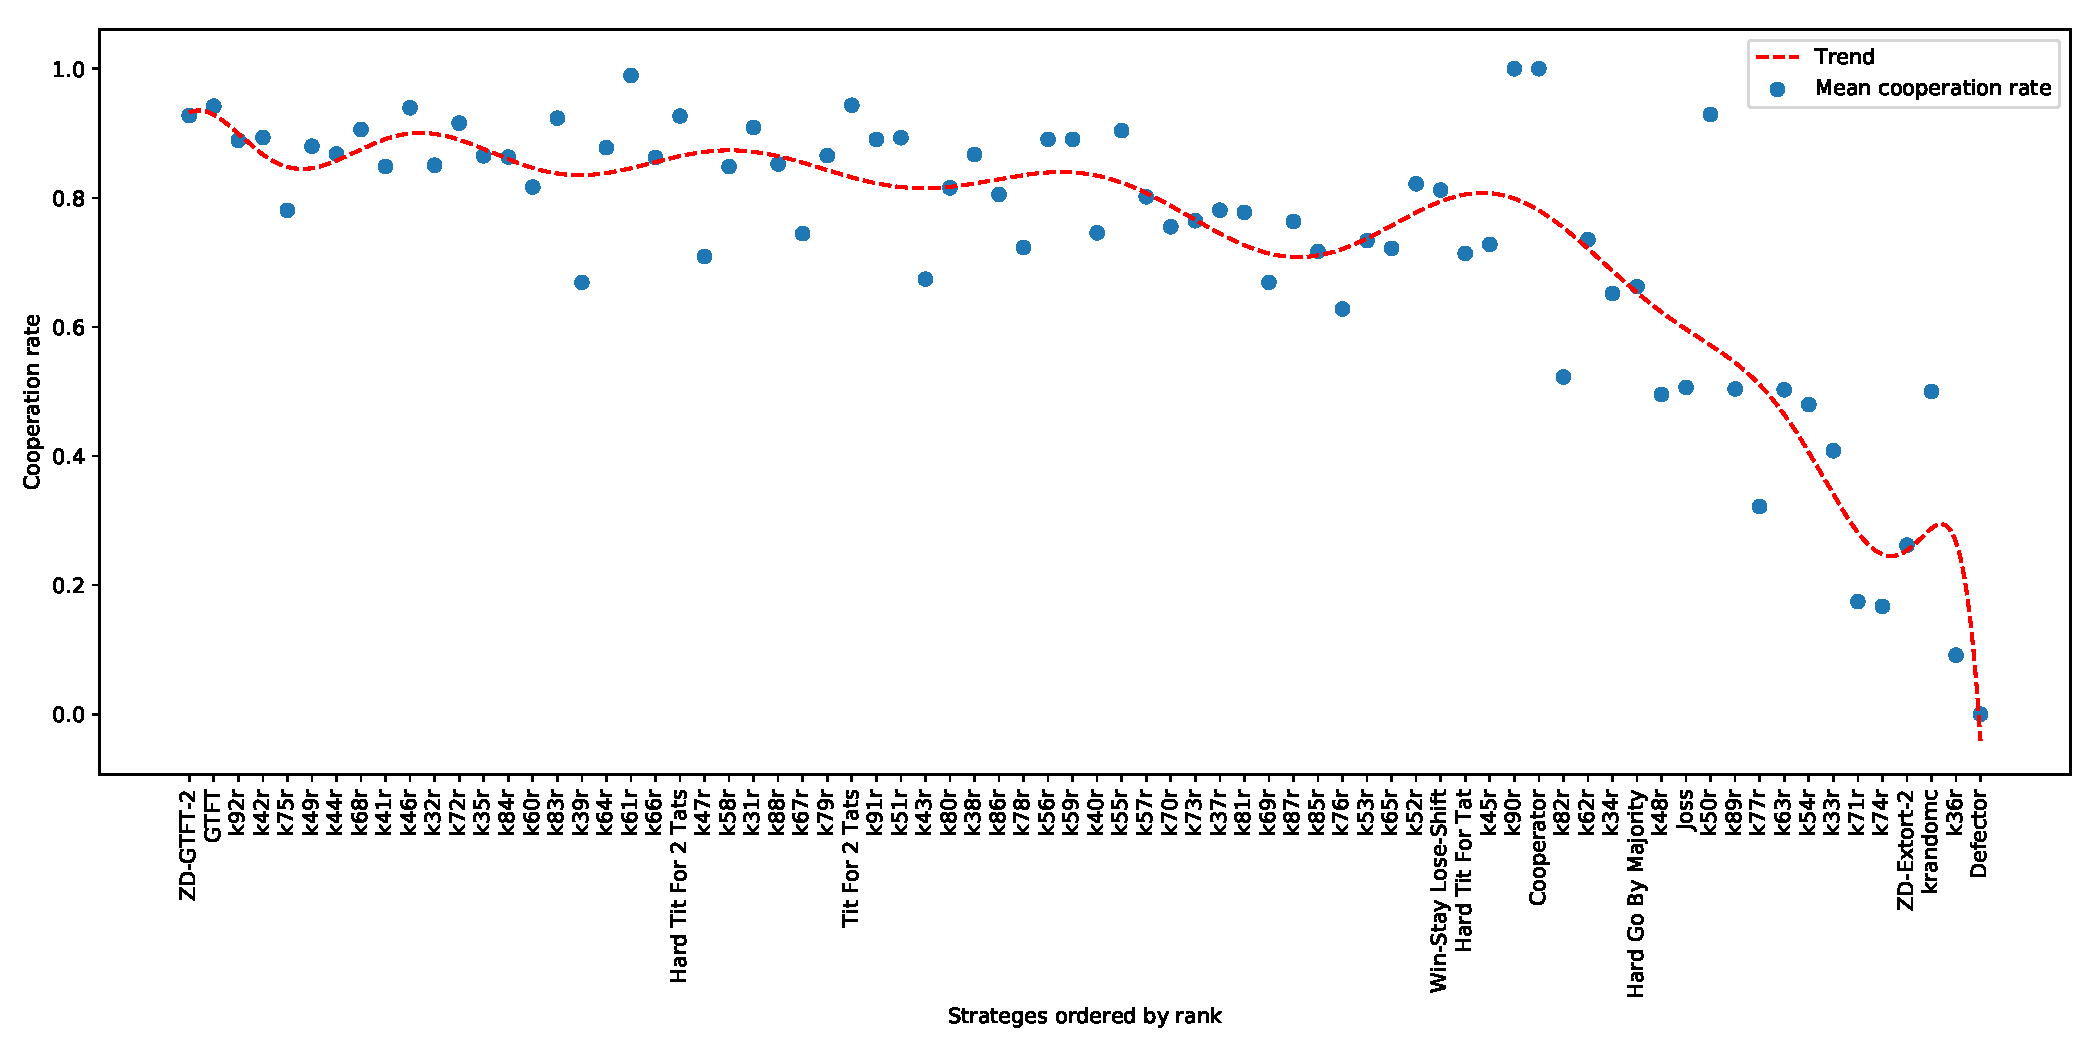
\includegraphics[width=.8\textwidth]{assets/sp_tournament_cooperation_rate_versus_rank.pdf}
    \caption{Cooperation rate versus rank for the Stewart and Poltkin tournament}
    \label{fig:sp_tournament_cooperation_rate_versus_rank}
\end{figure}


\begin{figure}[!hbtp]
    \centering
    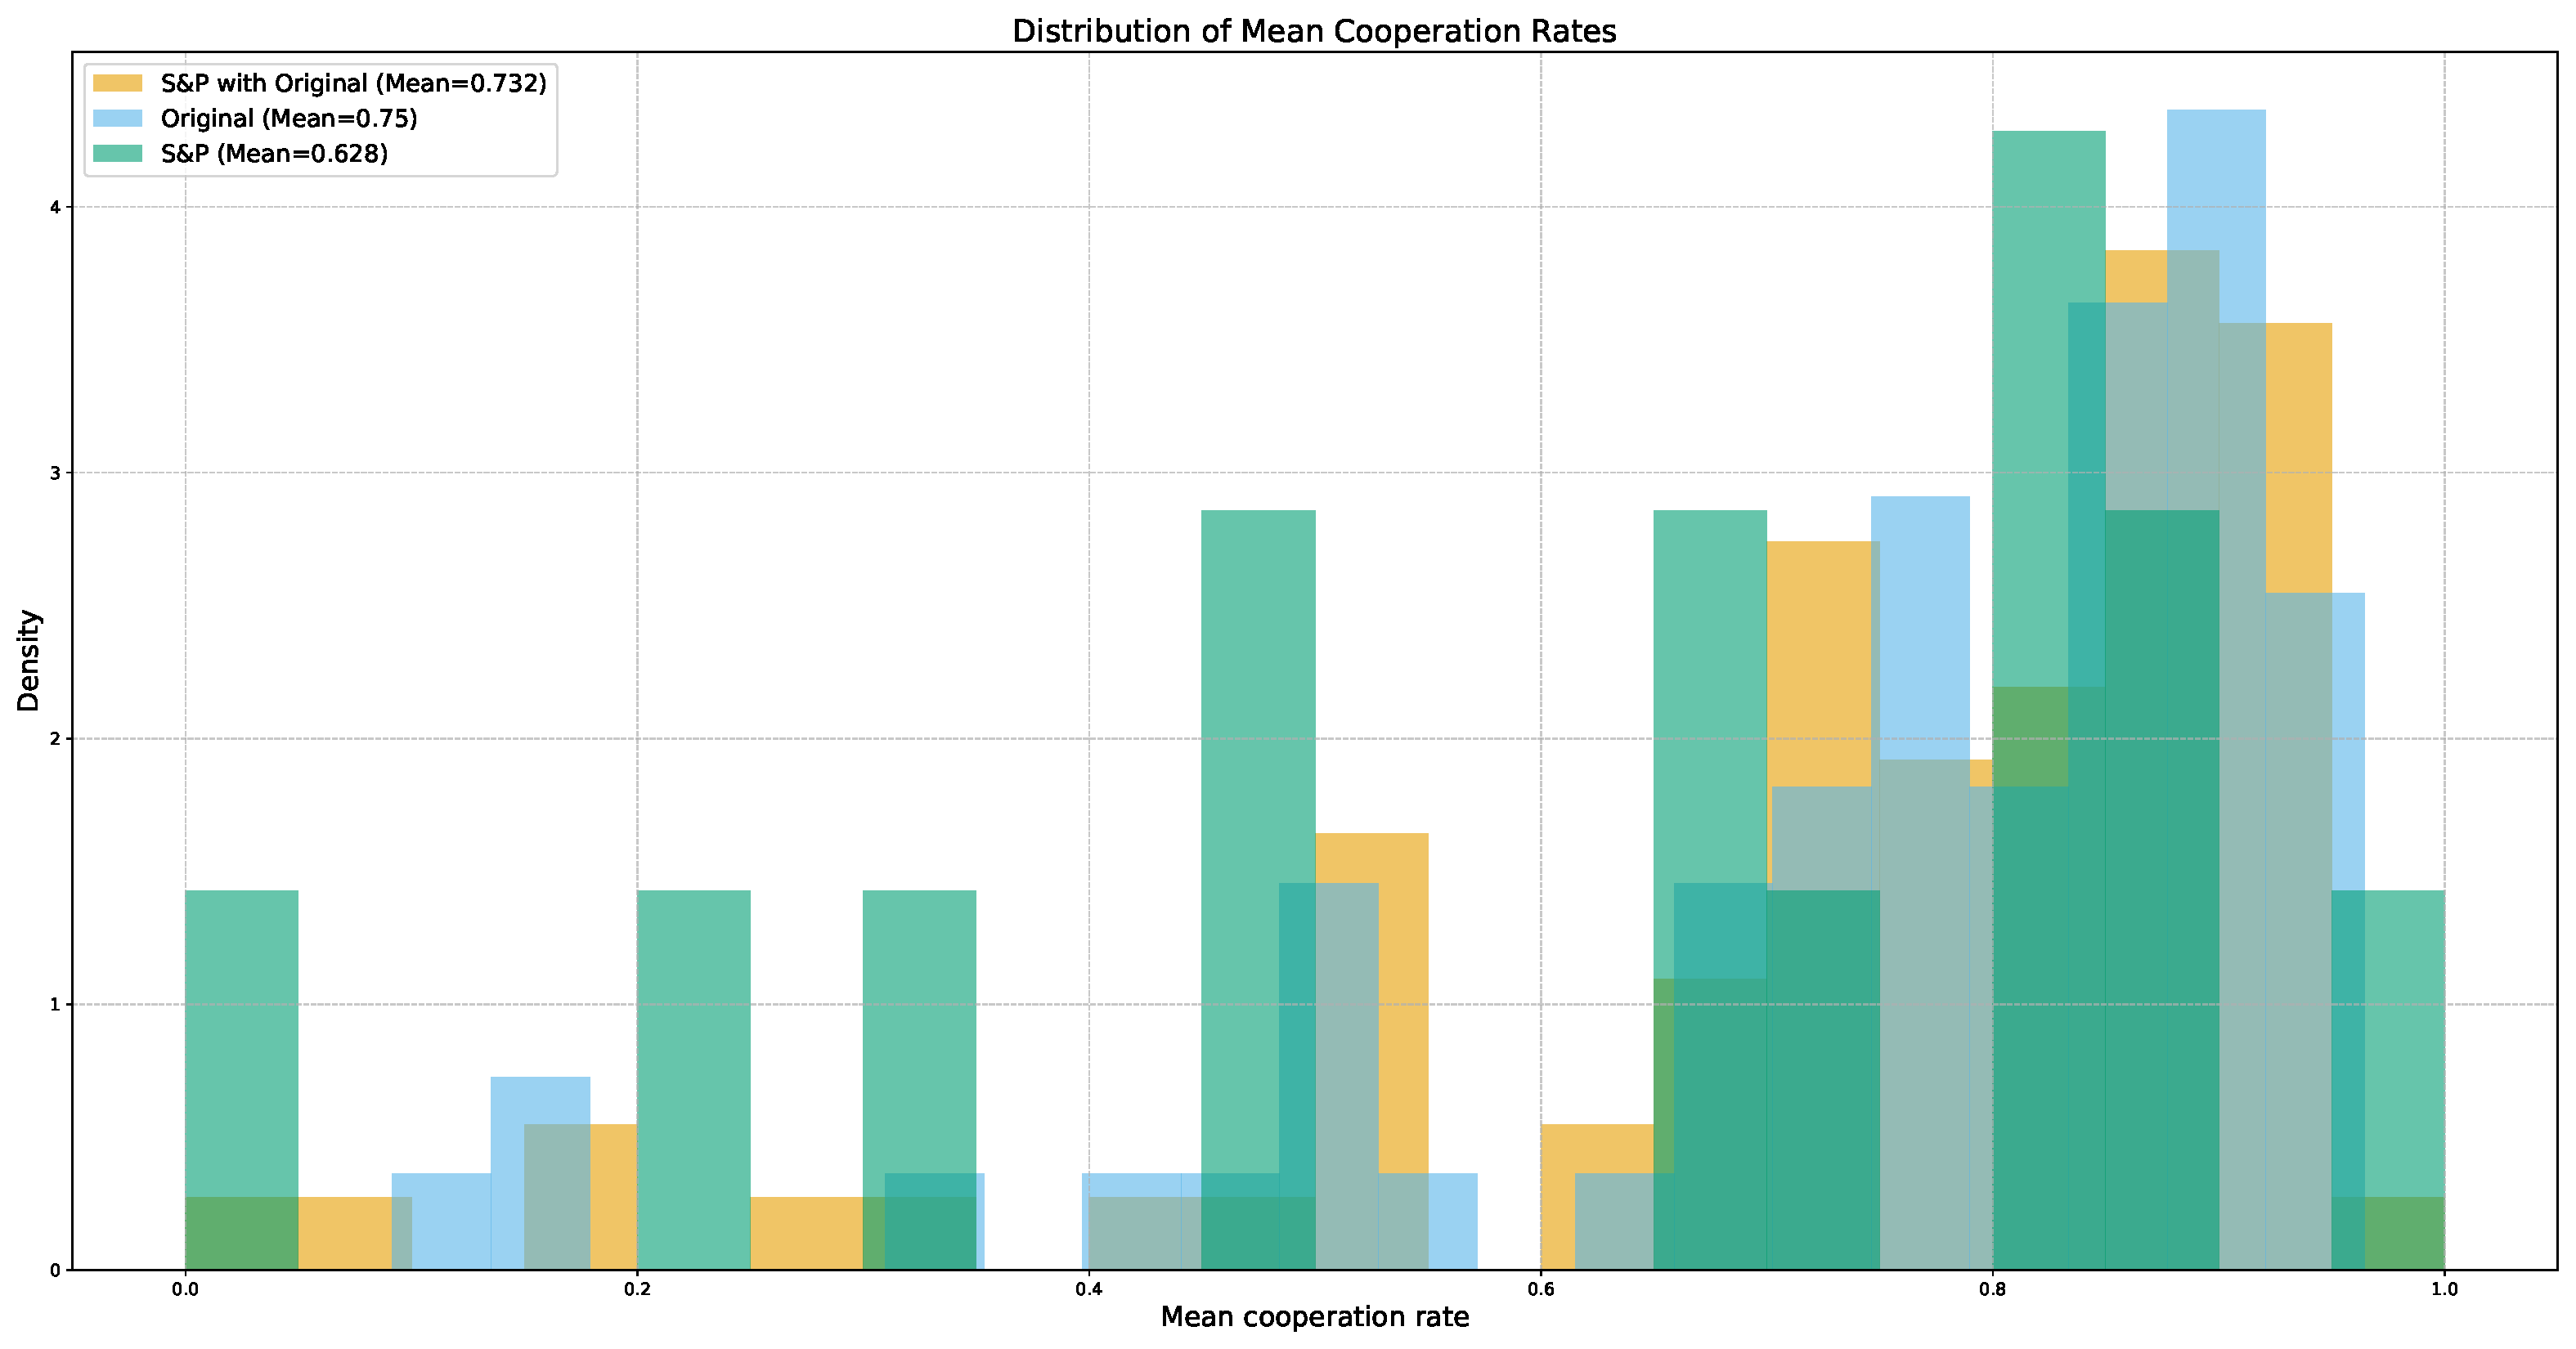
\includegraphics[width=.8\textwidth]{assets/sp_tournament_cooperation_rates.pdf}
    \caption{Distribution of cooperation rates for the Stewart and Plotkin
    tournament}
    \label{fig:sp_tournament_cooperation_rates}
\end{figure}

Figure~\ref{fig:sp_tournament_pairwise_cooperation_rates} shows the pair wise
cooperation rates.

\begin{figure}[!hbtp]
    \centering
    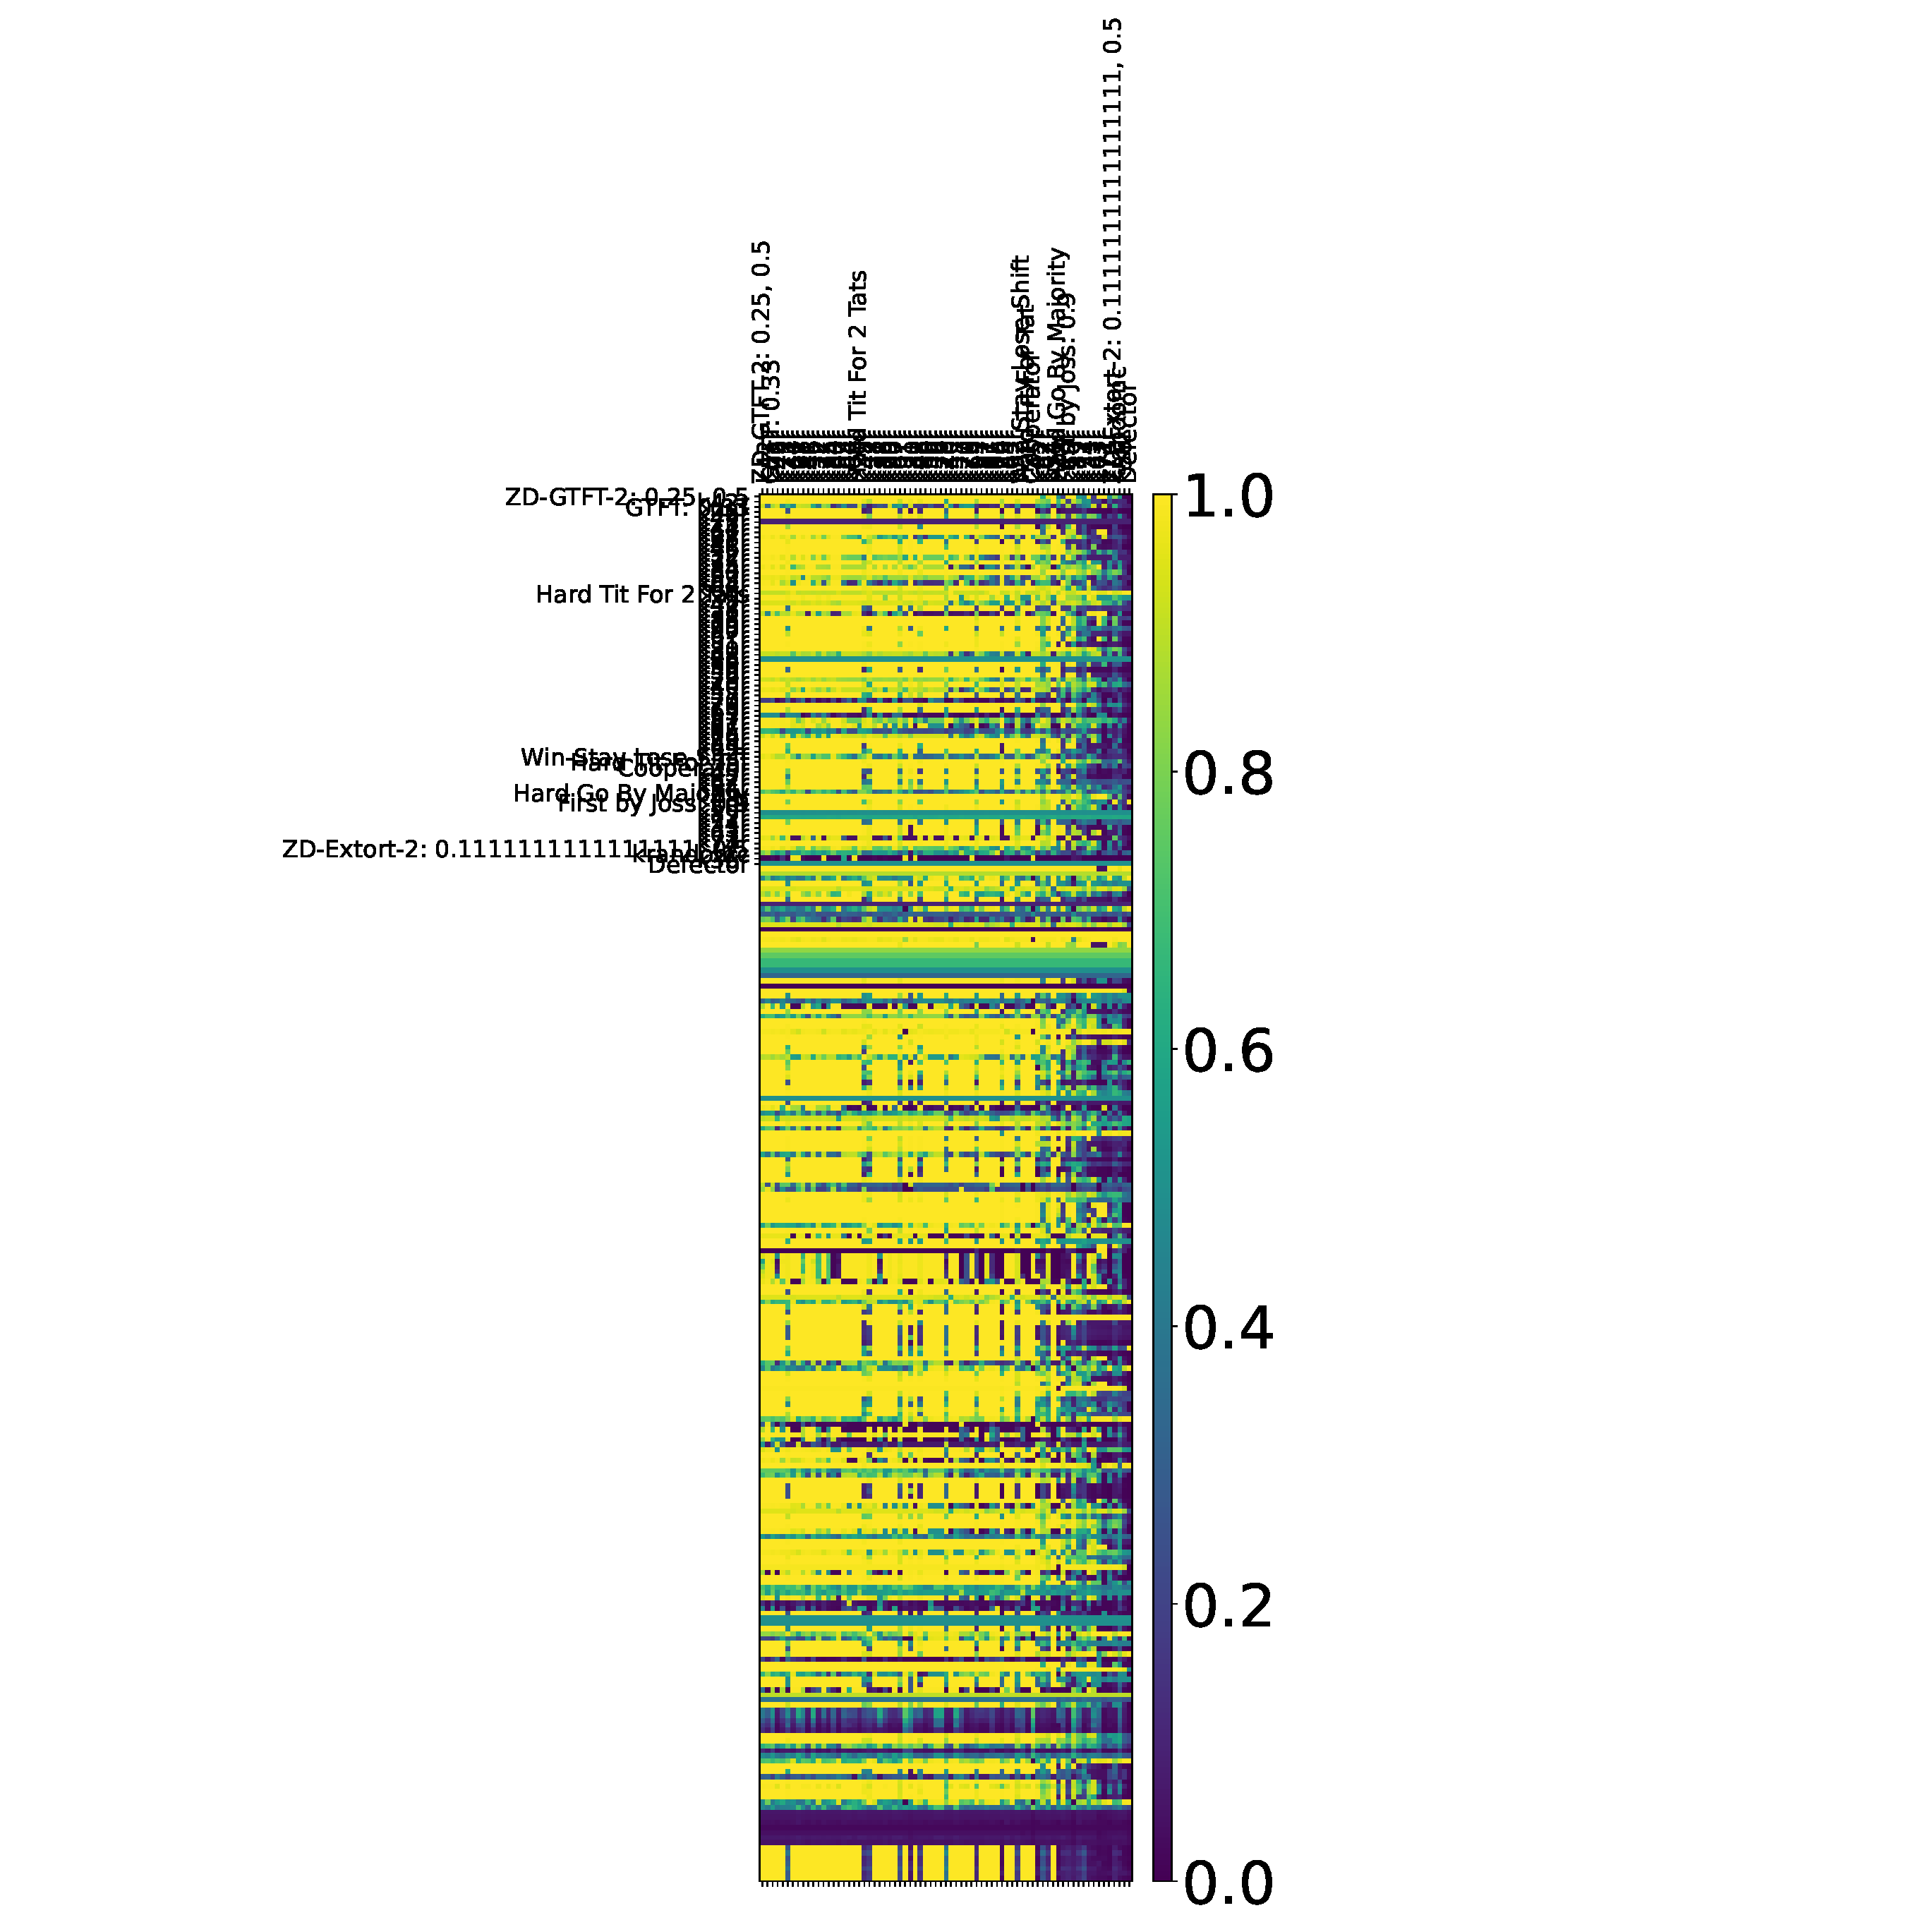
\includegraphics[width=.8\textwidth]{assets/sp_tournament_pairwise_cooperation_rates}
    \caption{Cooperation rates between each pair of players (ordered by rank)
    for the Stewart and Plotkin tournament}
    \label{fig:sp_tournament_pairwise_cooperation_rates}
\end{figure}

\subsubsection{Running a large tournament}\label{sec:run_with_everyone}

Table~\ref{tbl:full_tournament_rankings}
shows the rankings of the top 20 strategies when including all strategies over
4750repetitions.
The cooperation rate for the tournament that pits all the library strategies
against each other (without the Fortran ones) is
0.624\unskip.

\begin{table}[!hbtp]
        \centering
        \footnotesize
        \begin{tabular}{lrrrrrrr}
\toprule
 & Mean Score & Rank & Coop. Rate & Original Rank & Original Coop. Rate & Library Rank & Library Coop. Rate \\
\midrule
EvolvedLookerUp2\_2\_2 & 2.802 & 1 & 0.756 & NA & NA & 1 & 0.736 \\
Evolved HMM 5 & 2.788 & 2 & 0.751 & NA & NA & 2 & 0.742 \\
Omega TFT: 3, 8 & 2.786 & 3 & 0.750 & NA & NA & 12 & 0.725 \\
Evolved ANN 5 & 2.784 & 4 & 0.720 & NA & NA & 3 & 0.713 \\
Evolved ANN & 2.782 & 5 & 0.739 & NA & NA & 5 & 0.727 \\
Evolved FSM 16 & 2.780 & 6 & 0.731 & NA & NA & 4 & 0.713 \\
Evolved FSM 16 Noise 05 & 2.776 & 7 & 0.726 & NA & NA & 6 & 0.717 \\
PSO Gambler 2\_2\_2 & 2.760 & 8 & 0.702 & NA & NA & 7 & 0.692 \\
Original Gradual & 2.757 & 9 & 0.808 & NA & NA & NA & NA \\
PSO Gambler 2\_2\_2 Noise 05 & 2.756 & 10 & 0.740 & NA & NA & 14 & 0.723 \\
PSO Gambler Mem1 & 2.756 & 11 & 0.734 & NA & NA & 9 & 0.728 \\
Evolved FSM 4 & 2.752 & 12 & 0.793 & NA & NA & 10 & 0.777 \\
PSO Gambler 1\_1\_1 & 2.752 & 13 & 0.704 & NA & NA & 8 & 0.702 \\
Gradual & 2.746 & 14 & 0.763 & NA & NA & 15 & 0.793 \\
DBS: 0.75, 3, 4, 3, 5 & 2.739 & 15 & 0.750 & NA & NA & 11 & 0.739 \\
k42r & 2.735 & 16 & 0.820 & 3 & 0.916 & NA & NA \\
Winner12 & 2.733 & 17 & 0.688 & NA & NA & 16 & 0.682 \\
Spiteful Tit For Tat & 2.723 & 18 & 0.691 & NA & NA & 19 & 0.664 \\
k60r & 2.723 & 19 & 0.691 & 6 & 0.844 & NA & NA \\
k85r & 2.716 & 20 & 0.627 & 33 & 0.726 & NA & NA \\
EugineNier: (D,) & 2.713 & 21 & 0.673 & NA & NA & 22 & 0.645 \\
k80r & 2.706 & 22 & 0.723 & 36 & 0.809 & NA & NA \\
k32r & 2.704 & 23 & 0.758 & 10 & 0.873 & NA & NA \\
DoubleCrosser: (D, D) & 2.703 & 24 & 0.693 & NA & NA & 13 & 0.677 \\
k58r & 2.703 & 25 & 0.746 & 21 & 0.852 & NA & NA \\
\bottomrule
\end{tabular}

        \caption{Top 20 strategies in the tournament when using all available
        strategies}
        \label{tbl:full_tournament_rankings}
\end{table}

The overall cooperation rate of this tournament is
0.635and the various
cooperation rates are shown in
Figure~\ref{fig:full_tournament_cooperation_rate_versus_rank} shows the
cooperation rates of each strategy (ordered by rank).

\begin{figure}[!hbtp]
    \centering
    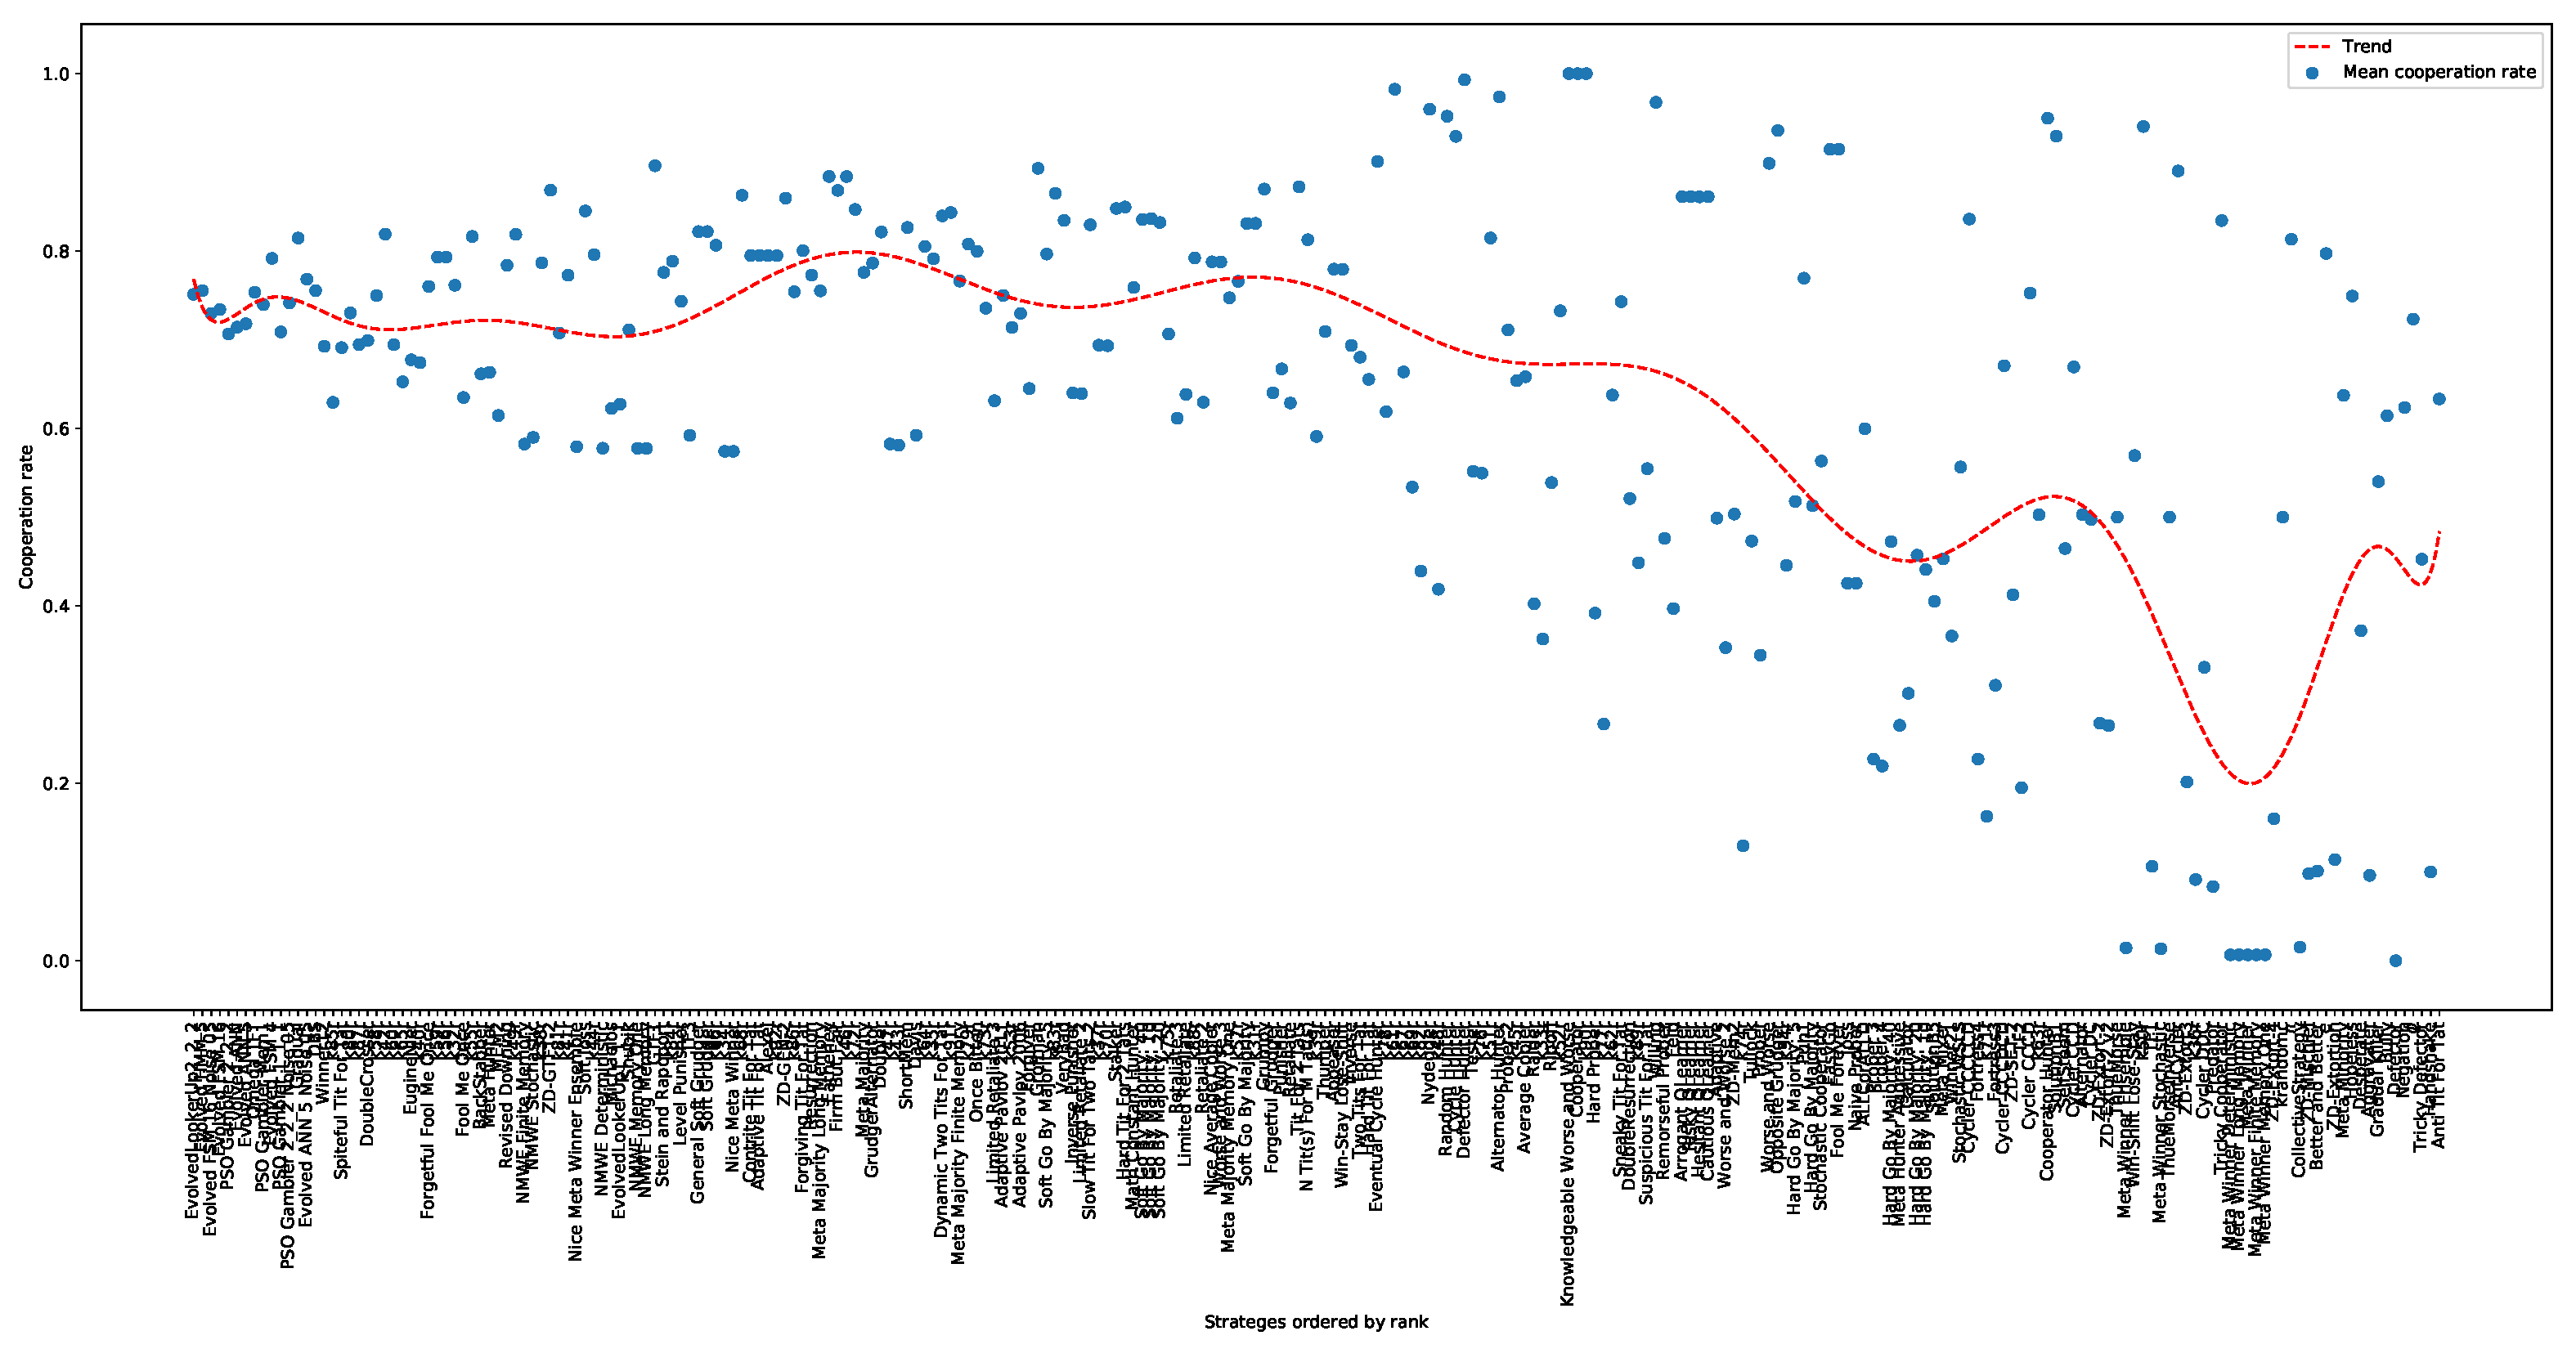
\includegraphics[width=.8\textwidth]{assets/full_tournament_cooperation_rate_versus_rank.pdf}
    \caption{Cooperation rate versus rank for tournament with all available
    strategies}
    \label{fig:full_tournament_cooperation_rate_versus_rank}
\end{figure}

\begin{figure}[!hbtp]
    \centering
    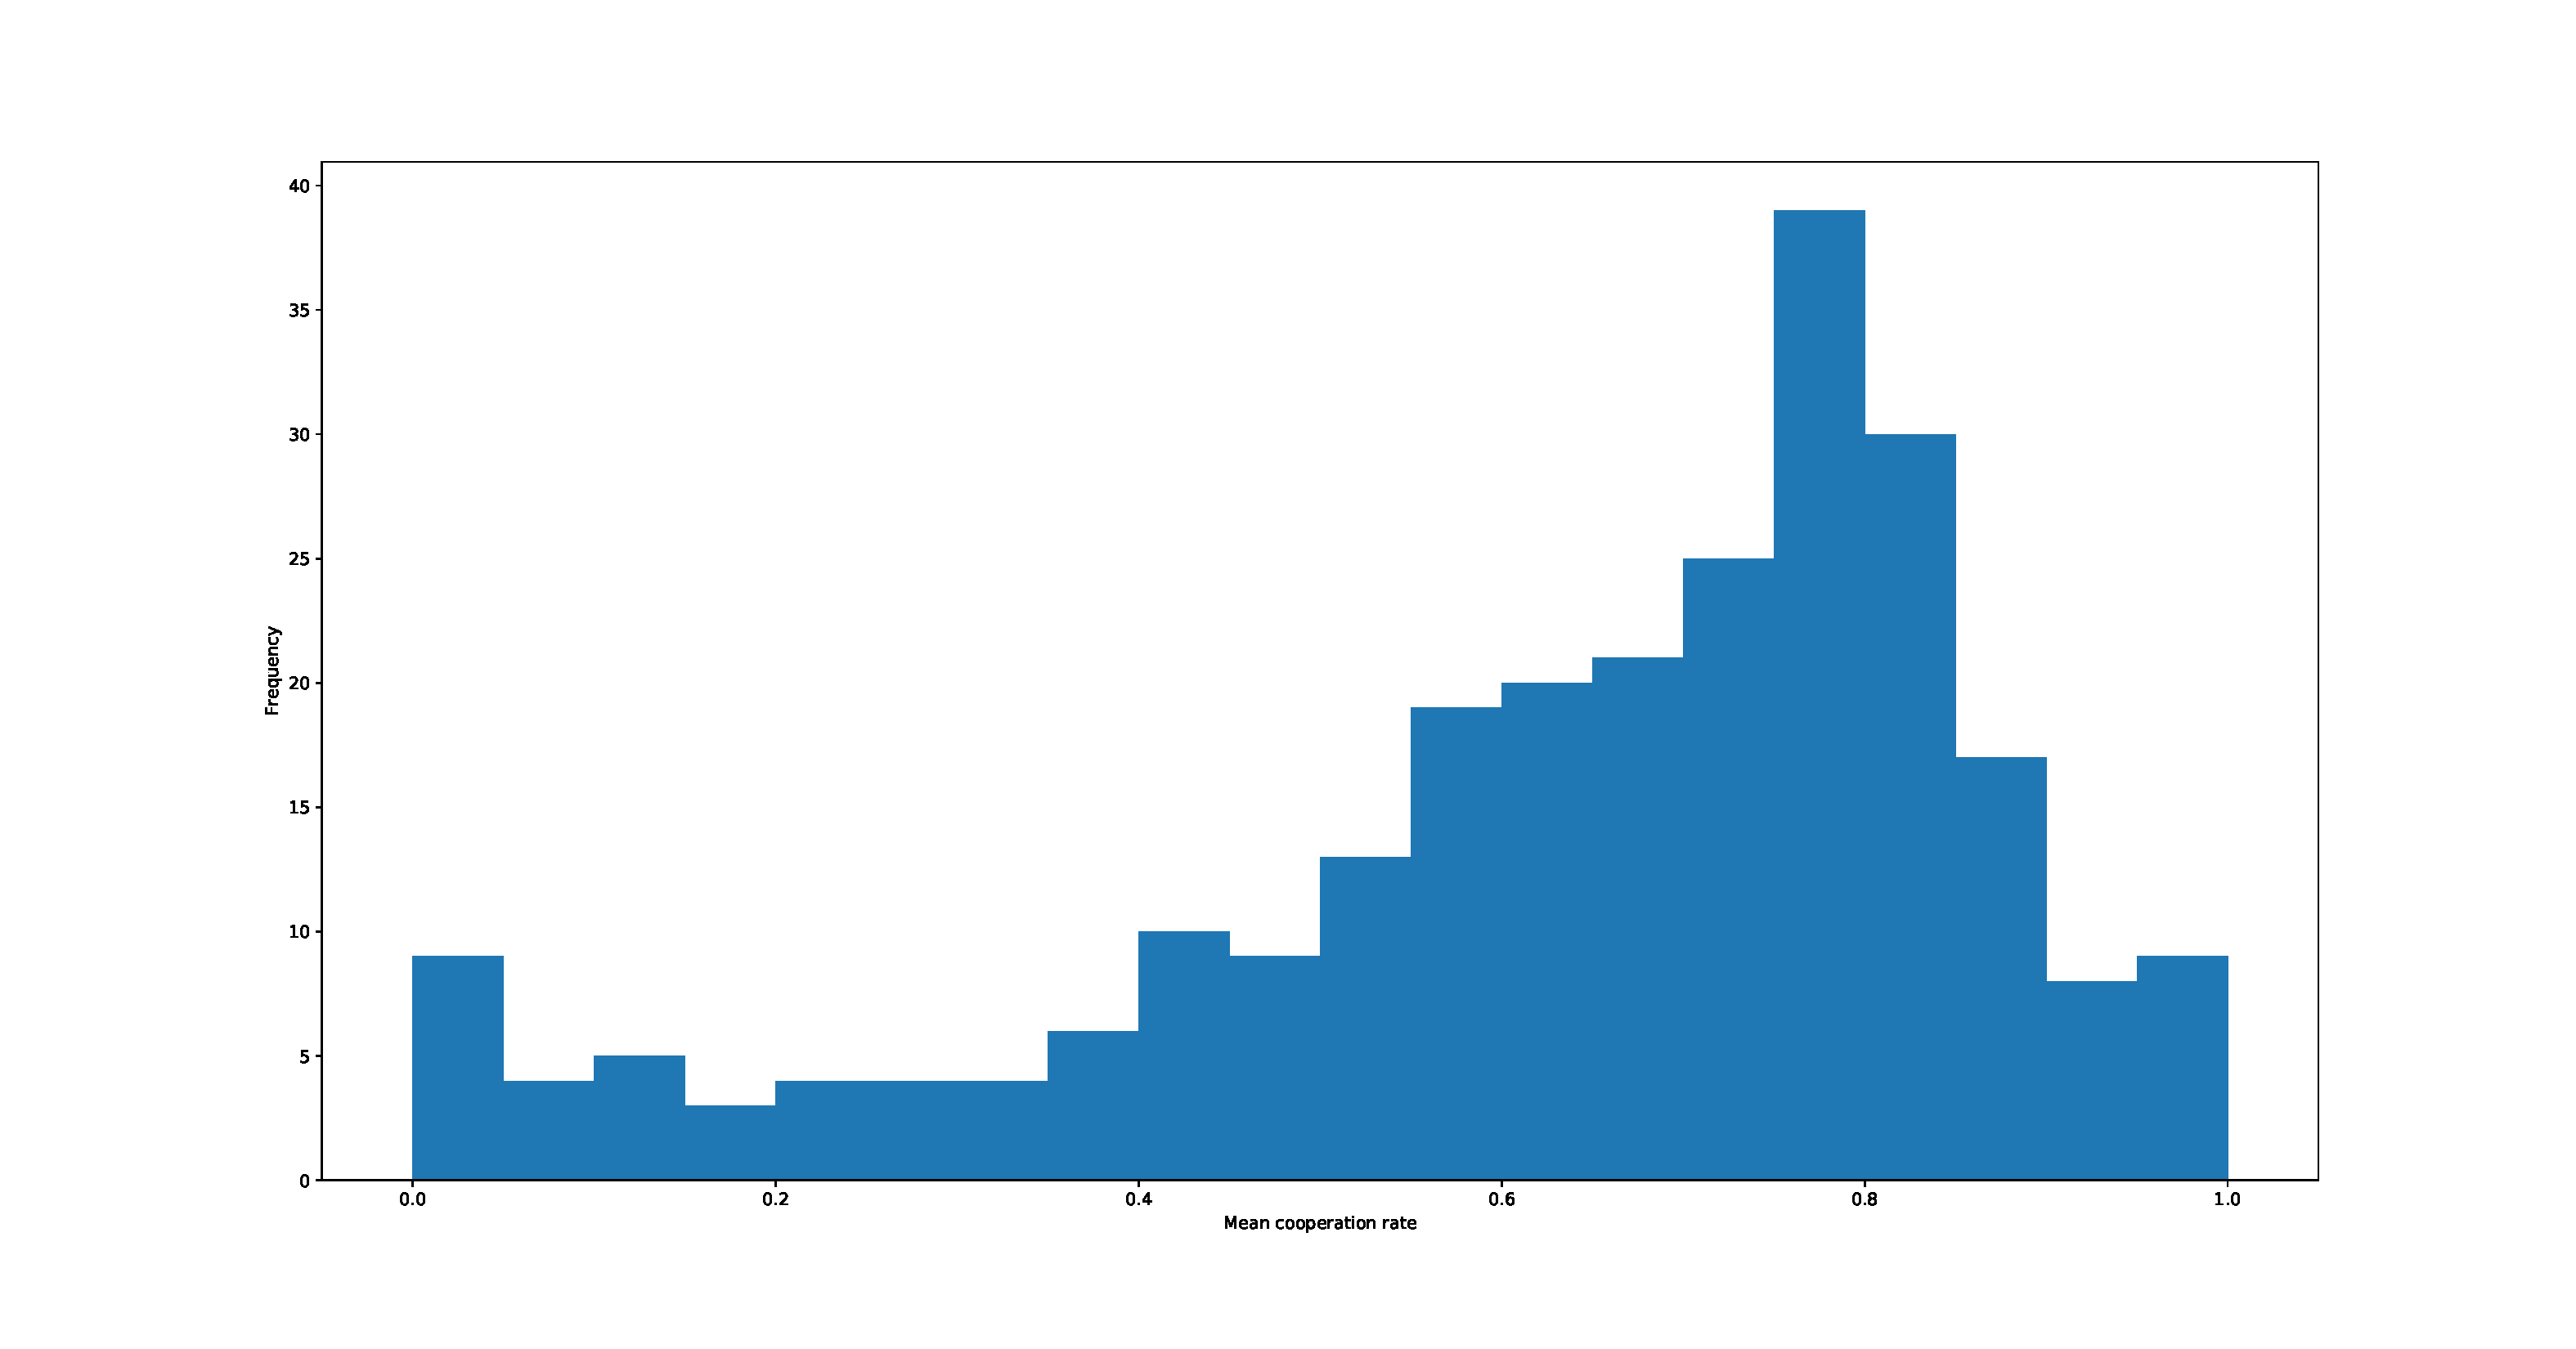
\includegraphics[width=.8\textwidth]{assets/full_tournament_cooperation_rates.pdf}
    \caption{Distribution of cooperation rates for the full tournament.}
    \label{fig:full_tournament_cooperation_rates}
\end{figure}

Figure~\ref{fig:full_tournament_pairwise_cooperation_rates} shows the pair wise
cooperation rates.

\begin{figure}[!hbtp]
    \centering
    \includegraphics[width=.8\textwidth]{assets/full_tournament_pairwise_cooperation_rates}
    \caption{Cooperation rates between each pair of players (ordered by rank)
    for tournament with all available strategies}
    \label{fig:full_tournament_pairwise_cooperation_rates}
\end{figure}

\section{Conclusion}\label{sec:conclusion}

\section*{Acknowledgements}

% TODO Write appendices for the Axelrod strategies

\bibliographystyle{plain}
\bibliography{bibliography.bib}

\appendix

\section{List of original players}\label{app:list_of_original_players}


\begin{multicols}{2}
    \begin{enumerate}
            \item k31r - Original rank: 23. Authored by Gail Grisell
\item k32r - Original rank: 10. Authored by Charles Kluepfel
\item k33r - Original rank: 59. Authored by Harold Rabbie
\item k34r - Original rank: 52. Authored by James W Friedman
\item k35r - Original rank: 11. Authored by Abraham Getzler
\item k36r - Original rank: 63. Authored by Roger Hotz
\item k37r - Original rank: 37. Authored by George Lefevre
\item k38r - Original rank: 34. Authored by Nelson Weiderman
\item k39r - Original rank: 25. Authored by Tom Almy
\item k40r - Original rank: 35. Authored by Robert Adams
\item k41r - Original rank: 7. Authored by Herb Weiner
\item k42r - Original rank: 3. Authored by Otto Borufsen
\item k43r - Original rank: 39. Authored by R D Anderson
\item k44r - Original rank: 5. Authored by William Adams
\item k45r - Original rank: 50. Authored by Michael F McGurrin
\item k46r - Original rank: 14. Authored by Graham J Eatherley
\item k47r - Original rank: 16. Authored by Richard Hufford
\item k48r - Original rank: 53. Authored by George Hufford
\item k49r - Original rank: 4. Authored by Rob Cave
\item k50r - Original rank: 54. Authored by Rik Smoody
\item k51r - Original rank: 18. Authored by John William Colbert
\item k52r - Original rank: 48. Authored by David A Smith
\item k53r - Original rank: 45. Authored by Henry Nussbacher
\item k54r - Original rank: 58. Authored by William H Robertson
\item k55r - Original rank: 42. Authored by Steve Newman
\item k56r - Original rank: 38. Authored by Stanley F Quayle
\item k57r - Original rank: 31. Authored by Rudy Nydegger
\item k58r - Original rank: 21. Authored by Glen Rowsam
\item k59r - Original rank: 40. Authored by Leslie Downing
\item k60r - Original rank: 6. Authored by Jim Graaskamp and Ken Katzen
\item k61r - Original rank: 2. Authored by Danny C Champion
\item k62r - Original rank: 51. Authored by Howard R Hollander
\item k63r - Original rank: 57. Authored by George Duisman
\item k64r - Original rank: 17. Authored by Brian Yamachi
\item k65r - Original rank: 47. Authored by Mark F Batell
\item k66r - Original rank: 20. Authored by Ray Mikkelson
\item k67r - Original rank: 27. Authored by Craig Feathers
\item k68r - Original rank: 12. Authored by Fransois Leyvraz
\item k69r - Original rank: 29. Authored by Johann Joss
\item k70r - Original rank: 32. Authored by Robert Pebly
\item k71r - Original rank: 60. Authored by James E Hall
\item k72r - Original rank: 13. Authored by Edward C White Jr
\item k73r - Original rank: 41. Authored by George Zimmerman
\item k74r - Original rank: 61. Authored by Edward Friedland
\item k75r - Original rank: 8. Authored by Paul D Harrington
\item k76r - Original rank: 46. Authored by David Gladstein
\item k77r - Original rank: 55. Authored by Scott Feld
\item k78r - Original rank: 19. Authored by Fred Mauk
\item k79r - Original rank: 26. Authored by Dennis Ambuehl and Kevin Hickey
\item k80r - Original rank: 36. Authored by Robyn M Dawes and Mark Batell
\item k81r - Original rank: 43. Authored by Martyn Jones
\item k82r - Original rank: 49. Authored by Robert A Leyland
\item k83r - Original rank: 15. Authored by Paul E Black
\item k84r - Original rank: 9. Authored by T Nicolaus Tideman and Paula Chieruzz
\item k85r - Original rank: 33. Authored by Robert B Falk and James M Langsted
\item k86r - Original rank: 28. Authored by Bernard Grofman
\item k87r - Original rank: 44. Authored by E E H Schurmann
\item k88r - Original rank: 22. Authored by Scott Appold
\item k89r - Original rank: 56. Authored by Gene Snodgrass
\item k90r - Original rank: 24. Authored by John Maynard Smith
\item k91r - Original rank: 30. Authored by Jonathan Pinkley
\item k92r - Original rank: 1. Authored by Anatol Rapoport
\item krandomc - Original rank: 62. Authored by None

    \end{enumerate}
\end{multicols}


\end{document}
